\documentclass[conference]{IEEEtran}
\IEEEoverridecommandlockouts

\usepackage{cite}
\usepackage{amsmath,amssymb,amsfonts}
\usepackage{graphicx}
\usepackage{subcaption}
\usepackage{booktabs}
\usepackage{array}
\usepackage{url}
\usepackage{xcolor}
\usepackage[T1]{fontenc}

\graphicspath{{../results/figures/}}

\begin{document}

\title{Performance of Missing-Data IAA Versus SNR\\in Synthesized Two-Reflector OCT Wedge Scans}

\author{
  \IEEEauthorblockN{Begaly Berimbay}
  \IEEEauthorblockA{
    \textit{Computational Optics for Biophotonic Imaging Lab (COBI)}\\
    Summer Internship Report\\
    \today
  }
}

\maketitle

%------------------------------------------------------------------
\begin{abstract}
This paper reports a simulator study of the Missing-data Iterative
Adaptive Approach (MIAA) applied to synthetic OCT fringes generated
from two equal-amplitude point reflectors whose axial separation
decreases linearly across a 1024-A-line B-scan. Four reconstruction
methods are compared: given-band DFT, IAA, MIAA without tapering
(MIAA\textsubscript{raw}), and MIAA with squared-cosine edge tapering
(MIAA\textsubscript{tap}). A Monte Carlo sweep over 11 SNR levels from
10\,dB to 60\,dB, with 30 independent noise realizations per
condition, yields resolution probability curves, 90\%-threshold maps,
missing-spectrum NMSE, localization RMSE, and amplitude ratio error.
The measured bandwidth of 6.5\,nm at a 510\,nm center wavelength is
extrapolated by a factor of four (64\,$\to$\,256 spectral samples) to
a synthesized 26\,nm bandwidth. DFT resolution is SNR-independent and
stalls at 28\,\textmu m, matching the sinc-squared Rayleigh limit of
the 6.5\,nm band. MIAA\textsubscript{raw} first reaches 90\%
two-reflector resolution at 50\,dB SNR (12\,\textmu m) and achieves
5\,\textmu m at 55\,dB, saturating at the 4$\times$ extrapolation
Rayleigh limit. IAA on the given band alone requires 60\,dB to reach
5\,\textmu m. Below 45\,dB none of the adaptive methods achieves 90\%
resolution at any tested separation. Missing-spectrum NMSE improves
from approximately $-2$\,dB at 10\,dB SNR to $-16$\,dB at 60\,dB.
Localization RMSE stays below 0.5\,\textmu m for well-separated
reflectors at SNR\,$\geq$\,55\,dB and amplitude ratio error is below
1\,dB for separations above the resolution threshold.
\end{abstract}

\begin{IEEEkeywords}
optical coherence tomography, iterative adaptive approach, spectral
extrapolation, superresolution, missing data, axial resolution, SNR
\end{IEEEkeywords}

%------------------------------------------------------------------
\section{Introduction}

Optical coherence tomography (OCT) resolves axial tissue microstructure
by recording the interference fringe produced between a reference beam
and light backscattered from the sample~\cite{huang1991oct}. The axial
point-spread function (PSF) width is governed by the source bandwidth:
for a rectangular spectrum of wavelength extent $\Delta\lambda$ centered
at $\lambda_0$, the Rayleigh separation between two equal reflectors is
approximately
\begin{equation}
  \Delta z \approx \frac{\lambda_0^2}{2\,\Delta\lambda}.
  \label{eq:rayleigh}
\end{equation}
Broadening the measurable bandwidth therefore directly narrows the PSF,
but spectral coverage in practical instruments is constrained by
detector arrays, light-source tuning ranges, and data-transfer
bandwidth.

The Iterative Adaptive Approach (IAA) was introduced to OCT by Zhu
\emph{et al.}~\cite{zhu2012iaa} as an alternative to DFT
reconstruction. IAA treats the depth reflectivity as a set of complex
sinusoidal amplitudes and iteratively fits them to the measured fringe
under a non-parametric minimum mean-square-error (MMSE) criterion.
Because IAA is a superresolution spectral estimator, it can resolve
reflectors closer than the Rayleigh limit when SNR is sufficient. The
missing-data extension, MIAA, goes further: IAA is first run on the
measured spectral band, and the resulting reflectivity model is then
used to extrapolate unmeasured spectral regions via the MMSE
missing-data formula~\cite{stoica2009missing}. If the extrapolation is
accurate, the reconstructed PSF corresponds to the wider synthesized
bandwidth.

This work implements both methods from scratch and quantifies
two-reflector resolution probability as a function of SNR using the
wedge B-scan geometry of~\cite{zhu2012iaa}. The spectral coverage is
set so that the measured band (6.5\,nm) occupies only the central
quarter of a 26\,nm virtual bandwidth, giving an extrapolation factor
of four. The performance ceiling imposed by this geometry---and the SNR
at which MIAA approaches it---is the central question.

%------------------------------------------------------------------
\section{Signal Model}

\subsection{Wavenumber Grid}

The measured spectrum is parameterized using the centered wavenumber
$q = k - k_c$, where $k = 2\pi/\lambda$ and $k_c = 2\pi/\lambda_0$.
Accounting for the nonlinear $k$-to-$\lambda$ mapping, the measured
wavenumber span is
\begin{equation}
  \Delta k_\text{given}
  = \frac{2\pi}{\lambda_\text{short}}
  - \frac{2\pi}{\lambda_\text{long}},
\end{equation}
where $\lambda_\text{short} = \lambda_0 - \Delta\lambda/2 = 506.75$\,nm
and $\lambda_\text{long} = \lambda_0 + \Delta\lambda/2 = 513.25$\,nm.
This gives $\Delta k_\text{given} = 1.570\times10^5$\,rad\,m$^{-1}$
divided into $N_\text{given} = 64$ uniform samples with spacing
$\delta q = \Delta k_\text{given}/N_\text{given} = 2453$\,rad\,m$^{-1}$.

The full spectral grid of $N_\text{total} = 256$ samples is formed by
centering the 64 measured indices within the wider array; the remaining
192 samples constitute the missing spectral support. The synthesized
bandwidth of $256\,\delta q$ corresponds to an effective wavelength
span of approximately 26\,nm. For depth reconstruction, $N_\text{recon}
= 4096$ bins with spacing $\pi/(N_\text{recon}\,\delta q) \approx
0.31$\,\textmu m provide a display grid without increasing physical
resolution.

\subsection{Fringe Synthesis}

For two reflectors at depths $z_1$ and $z_2$ with complex amplitudes
$a_1$ and $a_2$, the normalized analytic fringe over the given band is
\begin{equation}
  y(q_n) = a_1 e^{-j2q_n z_1} + a_2 e^{-j2q_n z_2},
  \quad n = 0,\ldots,N_\text{given}-1.
  \label{eq:fringe}
\end{equation}
The round-trip carrier phases $e^{-j2k_c z_i}$ are absorbed into the
amplitudes during synthesis, so $q$ is the baseband coordinate. Both
amplitudes are set to unity, giving a nominal amplitude ratio of 0\,dB.

\subsection{Noise and SNR}

Additive complex circular Gaussian noise is generated as
\begin{equation}
  w[n] = \frac{u[n] + j\,v[n]}{\sqrt{2}},
  \quad u[n],v[n]\sim\mathcal{N}(0,\sigma^2),
\end{equation}
rescaled to achieve the prescribed SNR exactly:
\begin{equation}
  \mathrm{SNR}_\text{dB}
  = 10\log_{10}\!\left(\frac{\|y\|^2/N_\text{given}}{\sigma^2}\right).
\end{equation}
The noise vector is rescaled after generation so that $\|w\|^2$ equals
the target noise power to numerical precision. The noisy observation is
$\tilde{y} = y + w$, restricted to the $N_\text{given}$ measured
samples.

\subsection{Wedge Geometry}

Two reflectors are placed symmetrically about a center depth
$z_c = 400$\,\textmu m. The separation decreases linearly across the
1024-A-line B-scan from 29\,\textmu m at A-line~0 to 0\,\textmu m at
A-line~1023:
\begin{equation}
  z_{1,2}(i) = z_c \mp \frac{\mathrm{sep}(i)}{2},
  \quad \mathrm{sep}(i) = 29\!\left(1 - \frac{i}{1023}\right)\,\mu\mathrm{m}.
\end{equation}
Figures~\ref{fig:setup} and~\ref{fig:fringe_examples} illustrate the
wedge geometry, spectral band layout, and representative noisy fringes
at three SNR levels.

\begin{figure}[t]
  \centering
  \begin{subfigure}[b]{0.48\columnwidth}
    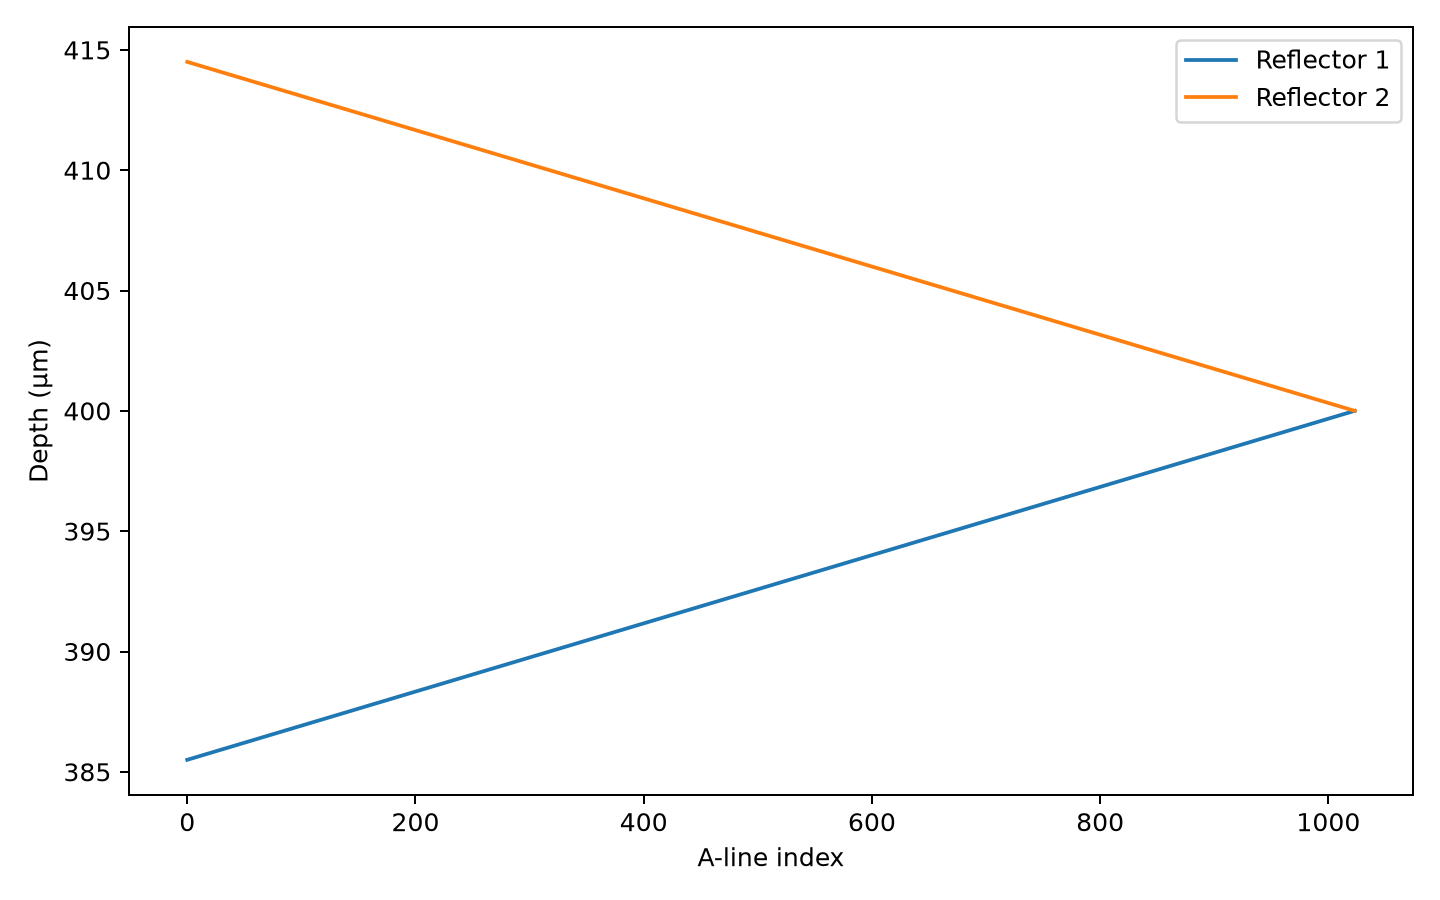
\includegraphics[width=\linewidth]{00_wedge_geometry}
    \caption{Wedge geometry}
  \end{subfigure}
  \hfill
  \begin{subfigure}[b]{0.48\columnwidth}
    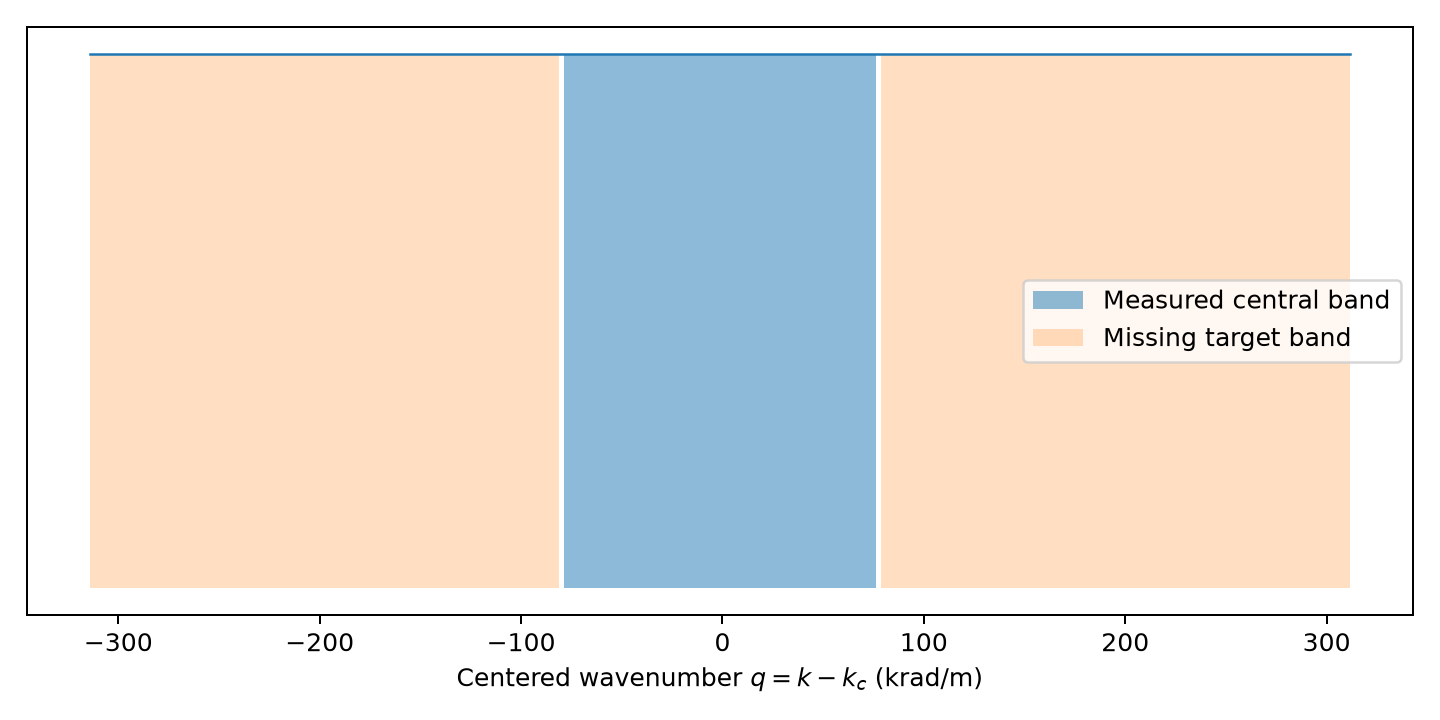
\includegraphics[width=\linewidth]{00_spectral_regions}
    \caption{Spectral band layout}
  \end{subfigure}
  \caption{Simulation setup. (a) Two reflectors approaching across the
    B-scan from 29\,\textmu m to 0\,\textmu m separation. (b) The
    64-sample measured band (blue) centered within the 256-sample
    virtual spectrum; the 192 missing samples (grey) are extrapolated
    by MIAA.}
  \label{fig:setup}
\end{figure}

\begin{figure}[t]
  \centering
  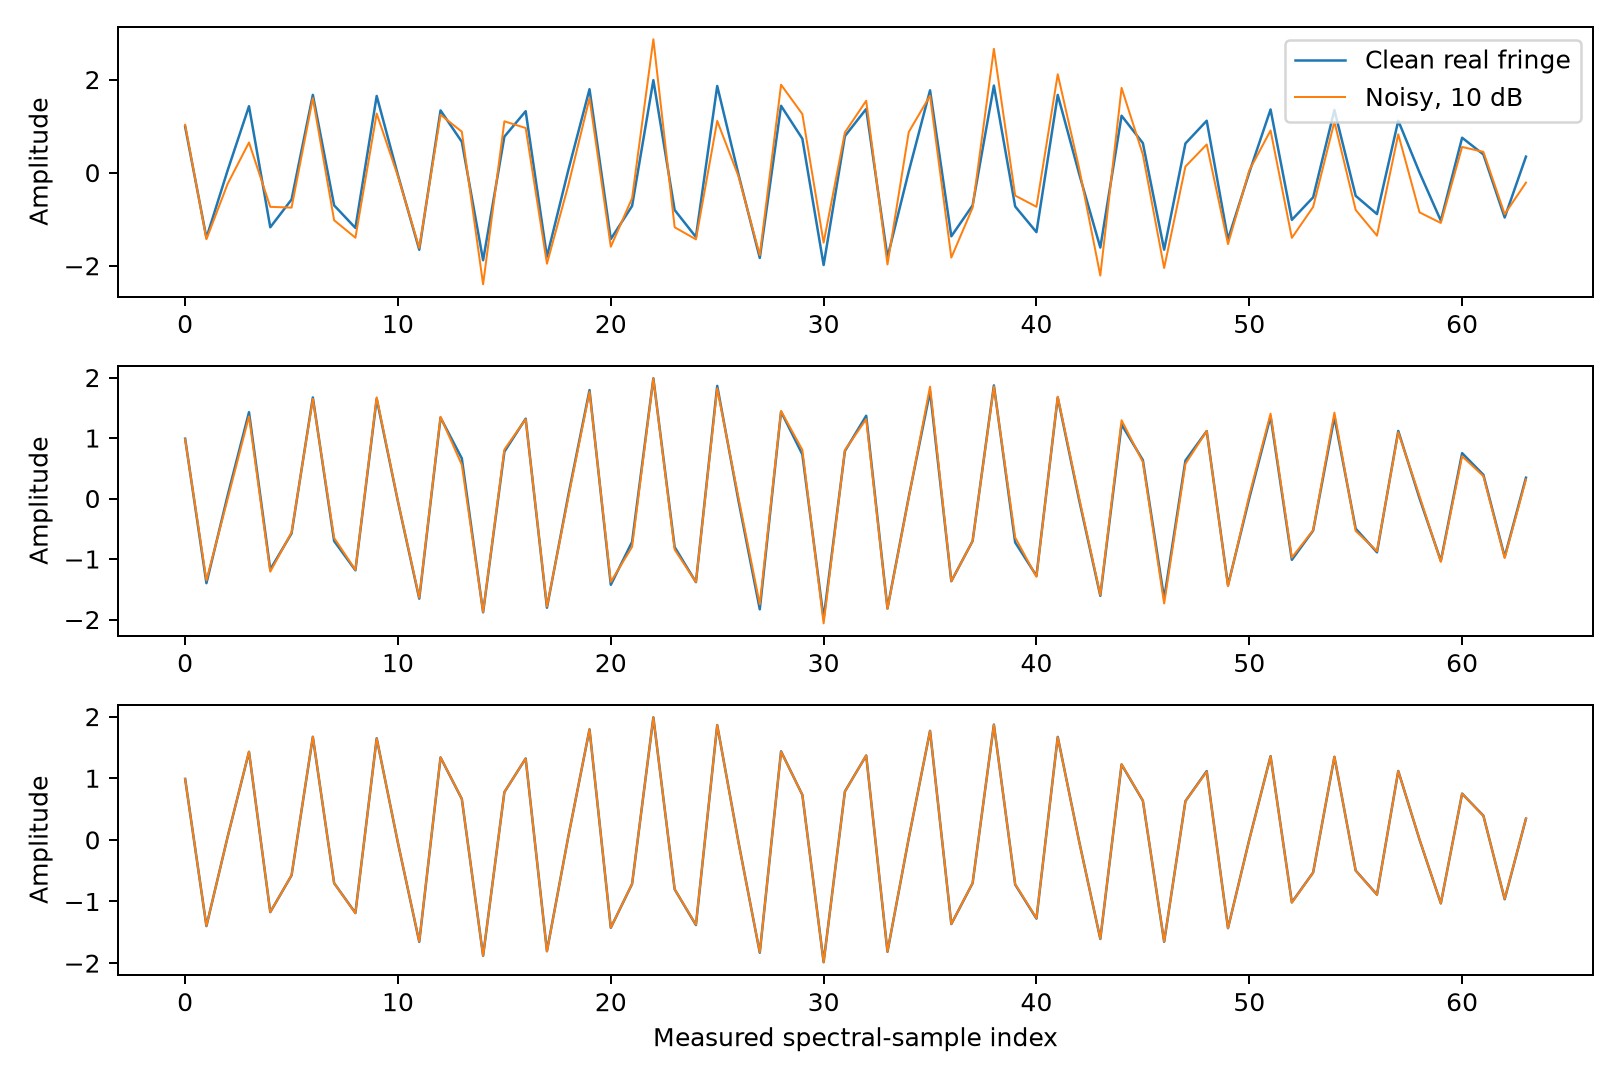
\includegraphics[width=\columnwidth]{00_noisy_fringe_examples}
  \caption{Noisy fringe realizations at SNR = 10, 30, and 50\,dB
    (reflector separation 15\,\textmu m). Noise visibly dominates the
    fringe at 10\,dB; the two-reflector beat pattern is recoverable
    only at high SNR.}
  \label{fig:fringe_examples}
\end{figure}

%------------------------------------------------------------------
\section{Reconstruction Methods}

\subsection{Given-Band DFT}

The baseline method zero-pads the $N_\text{given}$ measured samples
into an $N_\text{recon}$-point array (measured block centered) and
applies an $N_\text{recon}$-point IFFT without spectral tapering. The
resulting intensity profile has a sinc-squared PSF; applying the 3\,dB
valley criterion (Section~\ref{sec:design}) to this PSF yields an
observed DFT resolution threshold of 28\,\textmu m, consistent with
\eqref{eq:rayleigh} for a 6.5\,nm rectangular window.

\subsection{IAA on the Given Band}

IAA maintains a complex reflectivity vector
$\mathbf{a}\in\mathbb{C}^{N_\text{depth}}$ over a depth dictionary of
$N_\text{depth} = 512$ uniformly spaced depths in
$[300,500]$\,\textmu m. The Fourier basis matrix is
$\mathbf{F}_g\in\mathbb{C}^{N_\text{given}\times N_\text{depth}}$ with
entries
\begin{equation}
  [\mathbf{F}_g]_{n,\ell}
  = e^{-j2q_n z_\ell}.
\end{equation}

\subsubsection*{Initialization}
\begin{equation}
  \mathbf{a}^{(0)} = \mathbf{F}_g^H\tilde{y} / N_\text{given}.
\end{equation}

\subsubsection*{Covariance update}
\begin{equation}
  \mathbf{R}_g = \mathbf{F}_g\,\mathrm{diag}(|\mathbf{a}|^2)\,\mathbf{F}_g^H
  + \bigl(\sigma^2 + \varepsilon\,\max(\bar{r},1)\bigr)\mathbf{I},
  \label{eq:cov}
\end{equation}
where $\bar{r} = \mathrm{tr}(\mathbf{R}_g)/N_\text{given}$ is a
running scale estimate and $\varepsilon = 10^{-9}$ is a diagonal
loading factor. Before Cholesky factorization $\mathbf{R}_g$ is
replaced by $(\mathbf{R}_g + \mathbf{R}_g^H)/2$ to remove numerical
non-Hermitian round-off.

\subsubsection*{Reflectivity update}

Each depth index $\ell$ is updated as
\begin{equation}
  a_\ell^{(k+1)}
  = \frac{\mathbf{f}_{g,\ell}^H\,\mathbf{R}_g^{-1}\tilde{y}}
         {\mathbf{f}_{g,\ell}^H\,\mathbf{R}_g^{-1}\mathbf{f}_{g,\ell}},
  \label{eq:iaa_update}
\end{equation}
where $\mathbf{f}_{g,\ell}$ is the $\ell$-th column of
$\mathbf{F}_g$. The inversion $\mathbf{R}_g^{-1}$ is never formed
explicitly; $\mathbf{R}_g^{-1}\tilde{y}$ and
$\mathbf{R}_g^{-1}\mathbf{F}_g$ are computed via Cholesky
factorization. Ten cold iterations are used for the first A-line;
subsequent A-lines in the same sweep use two warm-start iterations
initialized from the previous A-line's reflectivity and covariance.

\subsection{MIAA Spectral Extrapolation}

After IAA converges, the missing spectral samples are estimated by the
MMSE formula~\cite{stoica2009missing}:
\begin{equation}
  \hat{y}_m
  = \mathbf{F}_m\,\mathrm{diag}(|\mathbf{a}|^2)\,
    \mathbf{F}_g^H\,\mathbf{R}_g^{-1}\tilde{y},
  \label{eq:miaa}
\end{equation}
where $\mathbf{F}_m\in\mathbb{C}^{N_\text{missing}\times N_\text{depth}}$
is the Fourier basis at the 192 missing wavenumbers. The measured
samples $\tilde{y}$ are copied unchanged. The full $N_\text{total}
= 256$-sample spectrum is assembled by inserting $\tilde{y}$ at the
given indices and $\hat{y}_m$ at the missing indices.

Two reconstructions are derived:
\begin{itemize}
  \item \textbf{MIAA\textsubscript{raw}}: zero-padded to $N_\text{recon}$
    and IFFTed without tapering.
  \item \textbf{MIAA\textsubscript{tap}}: a squared-cosine (Hann) taper
    applied to the outer 8\% of each spectral edge before IFFT, to
    suppress PSF sidelobes at the measured-to-extrapolated boundary.
\end{itemize}

\subsection{Oracle Full-Band DFT}

The clean noiseless fringe over all 256 samples is zero-padded to
$N_\text{recon}$ and IFFTed. This reference is unavailable in any real
system; it represents the resolution achievable if the full 26\,nm
band were measured noise-free.

%------------------------------------------------------------------
\section{Experimental Design}
\label{sec:design}

All parameters are drawn from \texttt{config\_final.yaml};
Table~\ref{tab:params} summarizes the complete parameter set.

\begin{table}[t]
  \caption{Simulation Parameters}
  \label{tab:params}
  \centering
  \renewcommand{\arraystretch}{1.15}
  \begin{tabular}{lc}
    \toprule
    Parameter & Value \\
    \midrule
    Center wavelength $\lambda_0$ & 510\,nm \\
    Measured bandwidth $\Delta\lambda$ & 6.5\,nm \\
    Measured samples $N_\text{given}$ & 64 \\
    Total spectral samples $N_\text{total}$ & 256 \\
    Extrapolation factor & 4$\times$ \\
    Reconstruction samples $N_\text{recon}$ & 4096 \\
    Depth dictionary $N_\text{depth}$ & 512 \\
    Depth range & 300--500\,\textmu m \\
    Center depth $z_c$ & 400\,\textmu m \\
    A-lines per B-scan & 1024 \\
    Maximum reflector separation & 29\,\textmu m \\
    Separation increment & 0.5\,\textmu m \\
    SNR levels tested & 10--60\,dB (11 levels) \\
    Monte Carlo seeds per SNR & 30 \\
    Cold IAA iterations & 10 \\
    Warm IAA iterations & 2 \\
    Diagonal loading $\varepsilon$ & $10^{-9}$ \\
    Edge taper fraction & 8\% \\
    Valley fraction criterion & 0.5 (3\,dB) \\
    Peak search window & $\pm$12\,\textmu m \\
    Localization tolerance & 5\,\textmu m \\
    Random seed & 2026 \\
    \bottomrule
  \end{tabular}
\end{table}

\textbf{Resolution criterion.} Two reflectors are considered resolved
if both conditions hold simultaneously:
\begin{enumerate}
  \item The intensity valley between the two PSF peaks falls to
    $\leq 50\%$ ($-3$\,dB) of the smaller peak intensity.
  \item The absolute localization error of each detected peak from its
    true depth is $\leq 5$\,\textmu m.
\end{enumerate}
The 90\%-resolution threshold is the smallest separation at which
resolution probability $\geq 0.90$, found by scanning from largest to
smallest separation; this prevents isolated spurious successes at small
separations from being counted as resolved.

The total Monte Carlo accounting is $11~\text{SNR}\times
30~\text{seeds}\times 59~\text{separations}\times 4~\text{methods}
= 77{,}880$ rows.

%------------------------------------------------------------------
\section{Validation}

\textbf{Single reflector.} A single reflector at $z = 400$\,\textmu m
was processed at 30\,dB SNR. The IAA-estimated depth agreed with the
true depth to within 0.3\,\textmu m and the MIAA missing-spectrum NMSE
was $-10.2$\,dB, consistent with the moderate-SNR regime.

\textbf{Two reflectors---separated.} At $\Delta z = 25$\,\textmu m and
30\,dB SNR (Fig.~\ref{fig:validation}a), both IAA and MIAA correctly
resolved the pair. Localization RMSE was 0.6\,\textmu m and amplitude
ratio error 0.3\,dB.

\textbf{Two reflectors---close.} At $\Delta z = 7$\,\textmu m and
50\,dB SNR (Fig.~\ref{fig:validation}b), DFT failed to resolve the
pair. MIAA\textsubscript{raw} successfully resolved both reflectors
with localization RMSE of 1.1\,\textmu m. IAA on the given band alone
failed to resolve, confirming that spectral extrapolation provides a
genuine benefit beyond superresolution within the measured band.

\begin{figure}[t]
  \centering
  \begin{subfigure}[b]{0.48\columnwidth}
    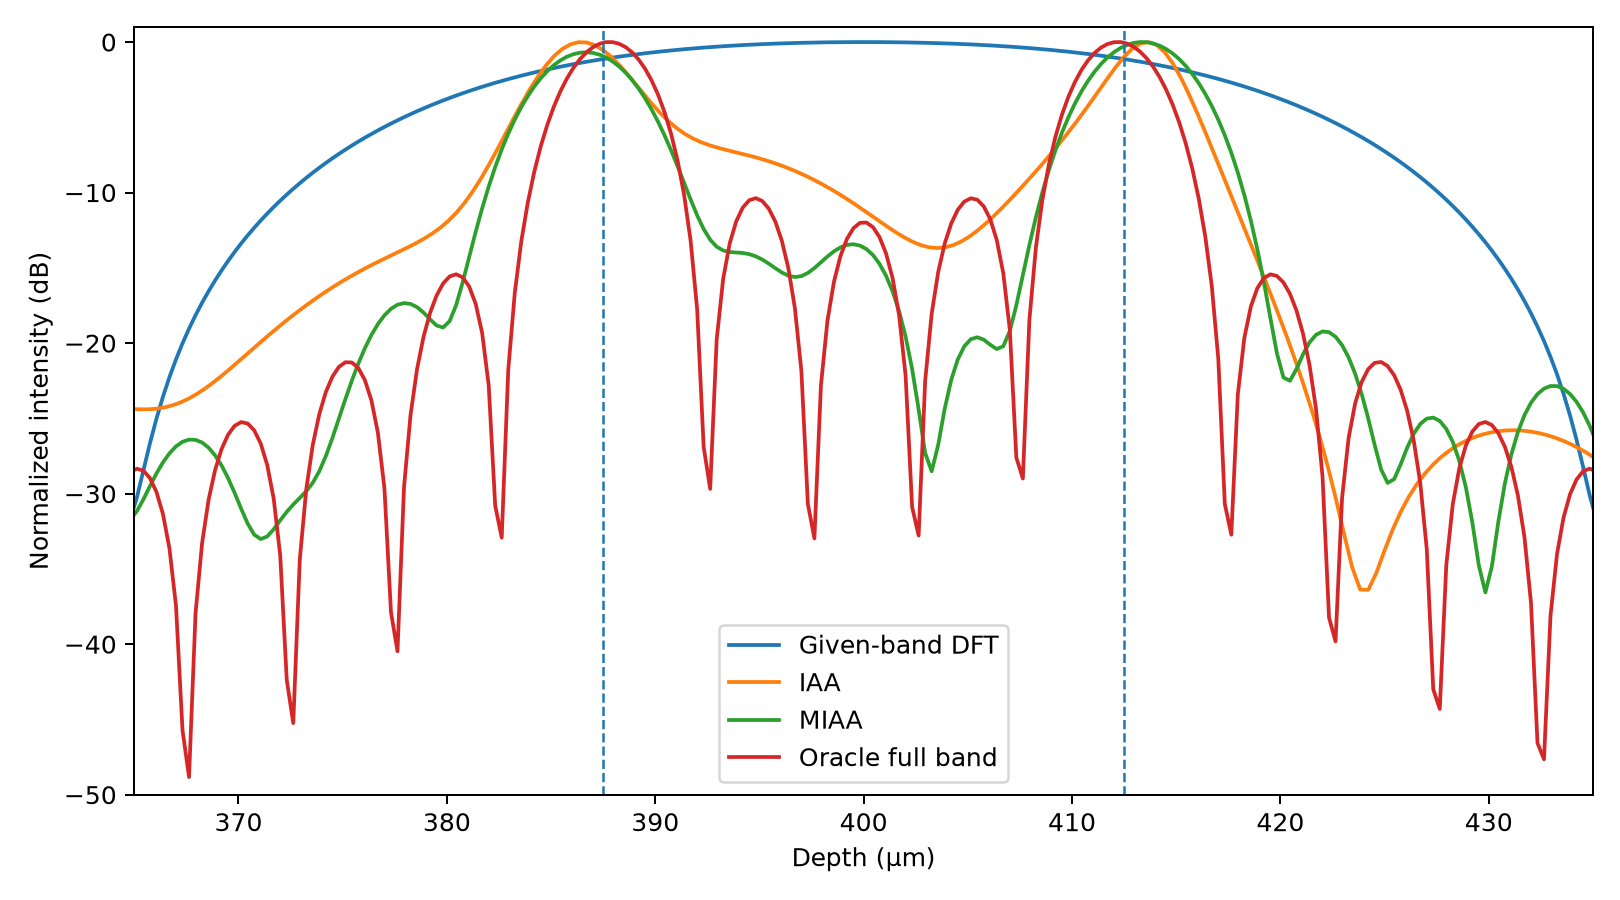
\includegraphics[width=\linewidth]{02_two_reflectors_25um}
    \caption{$\Delta z = 25$\,\textmu m, 30\,dB}
  \end{subfigure}
  \hfill
  \begin{subfigure}[b]{0.48\columnwidth}
    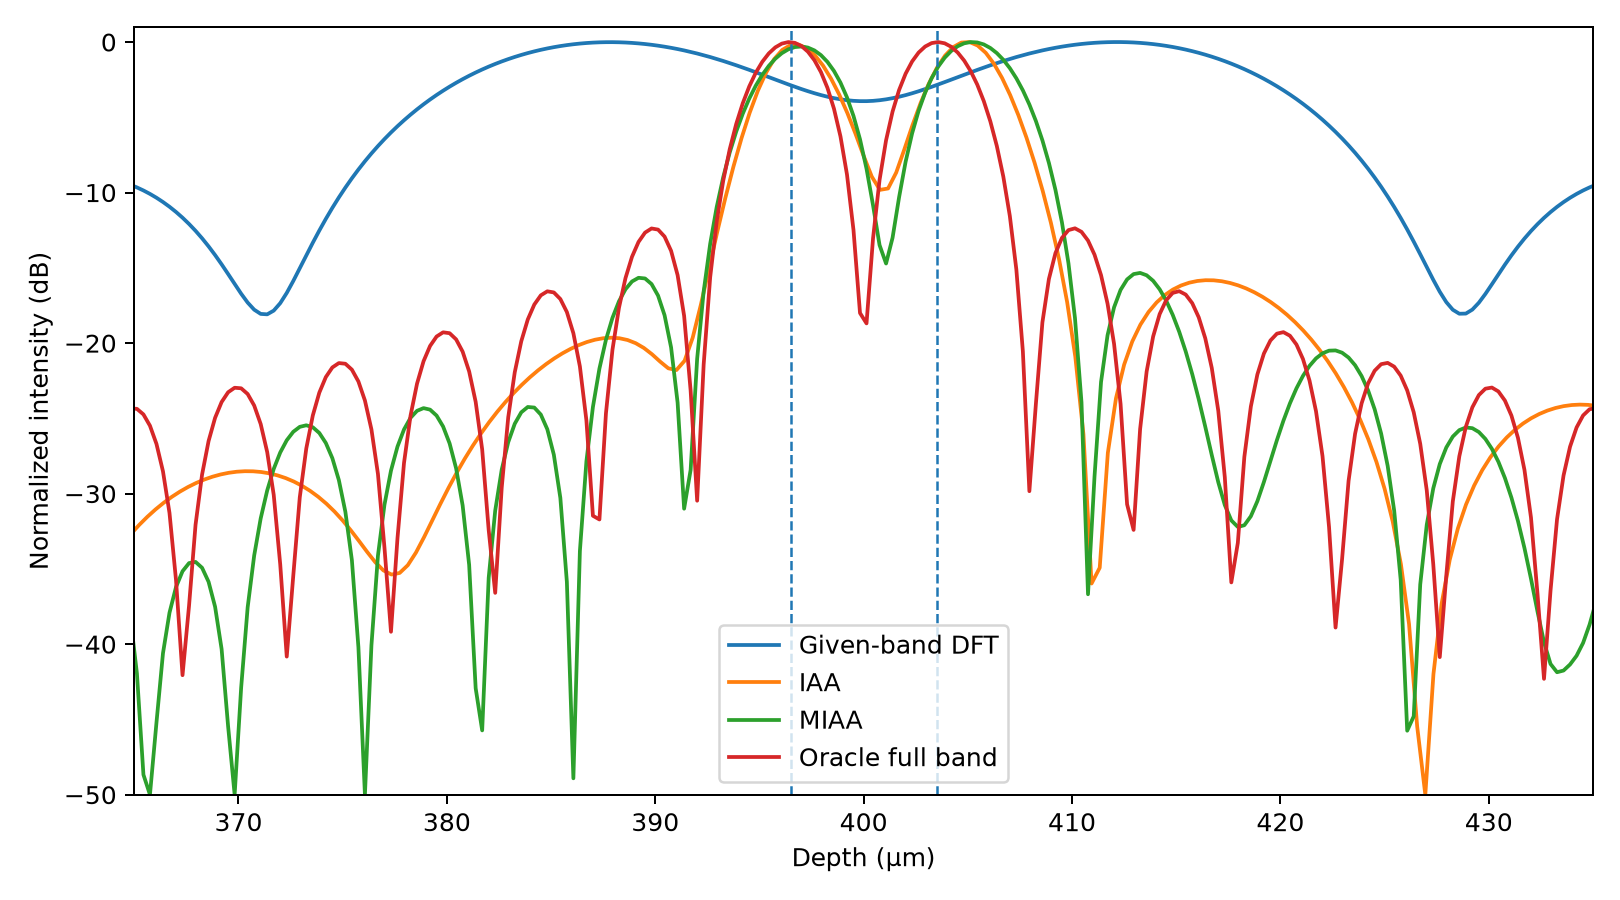
\includegraphics[width=\linewidth]{02_two_reflectors_7um}
    \caption{$\Delta z = 7$\,\textmu m, 50\,dB}
  \end{subfigure}
  \caption{Two-reflector validation. (a) Well-separated case: DFT,
    IAA, and MIAA all resolve the pair. (b) Sub-Rayleigh case: DFT
    fails; MIAA\textsubscript{raw} resolves both reflectors.}
  \label{fig:validation}
\end{figure}

%------------------------------------------------------------------
\section{Results}

\subsection{Representative Wedge B-Scans}

Figures~\ref{fig:bscan_10}--\ref{fig:bscan_50} show DFT, IAA, MIAA,
and oracle B-scans at SNR = 10, 30, and 50\,dB respectively. All
images are displayed as $10\log_{10}(I/I_\text{max})$ with a
$-45$\,dB floor.

\begin{figure}[htbp]
  \centering
  \begin{subfigure}[b]{0.48\columnwidth}
    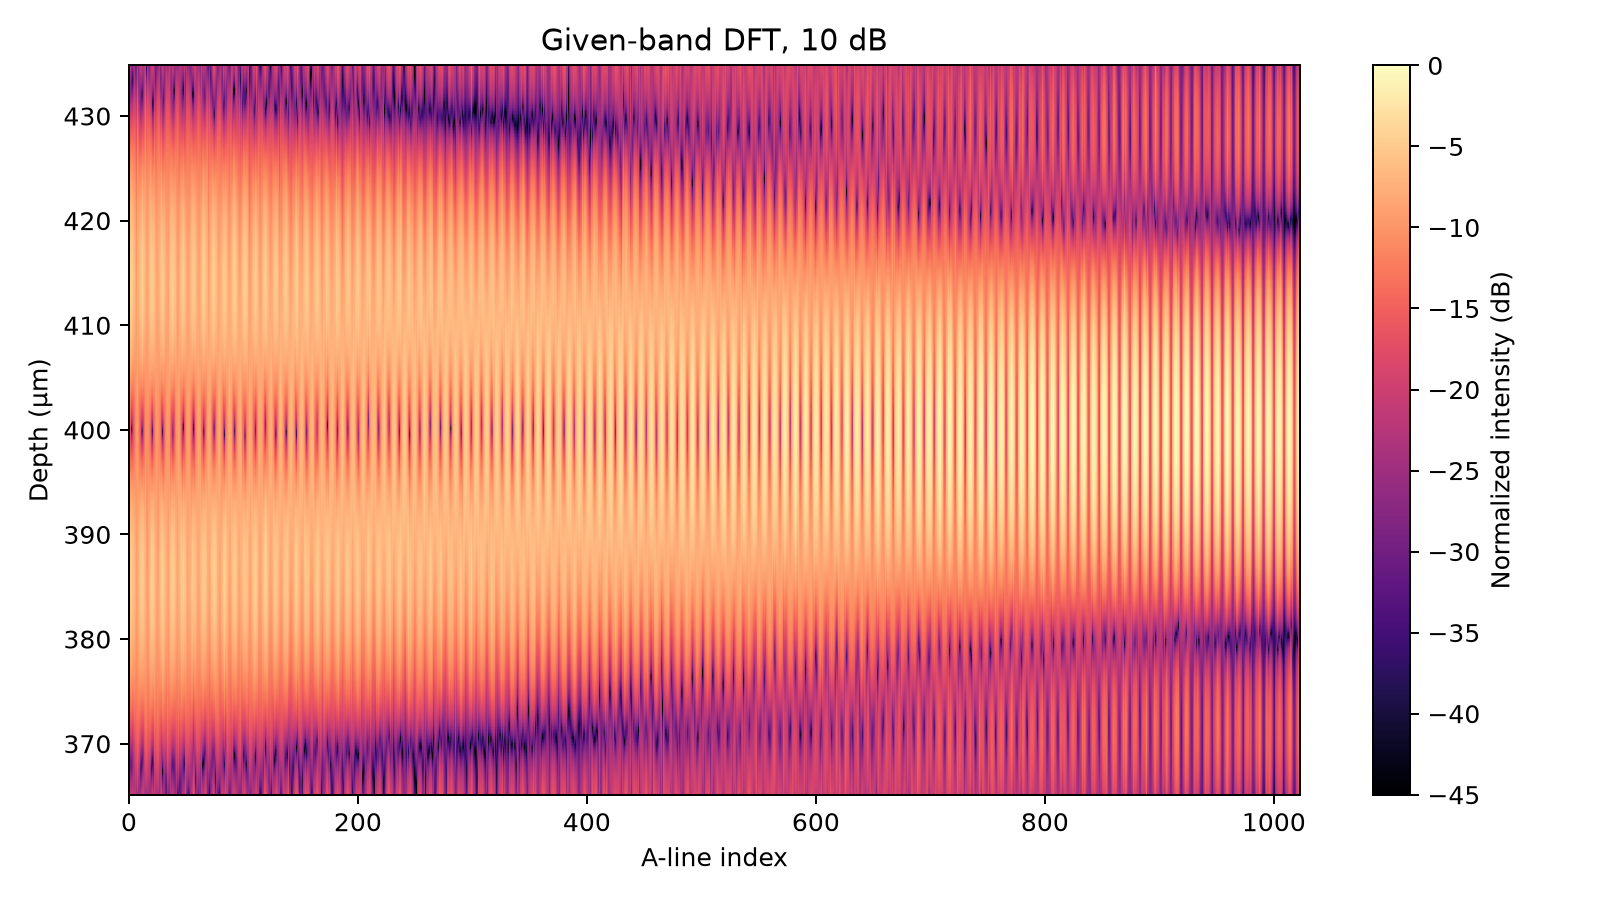
\includegraphics[width=\linewidth]{03_wedge_dft_10dB}
    \caption{DFT}
  \end{subfigure}
  \hfill
  \begin{subfigure}[b]{0.48\columnwidth}
    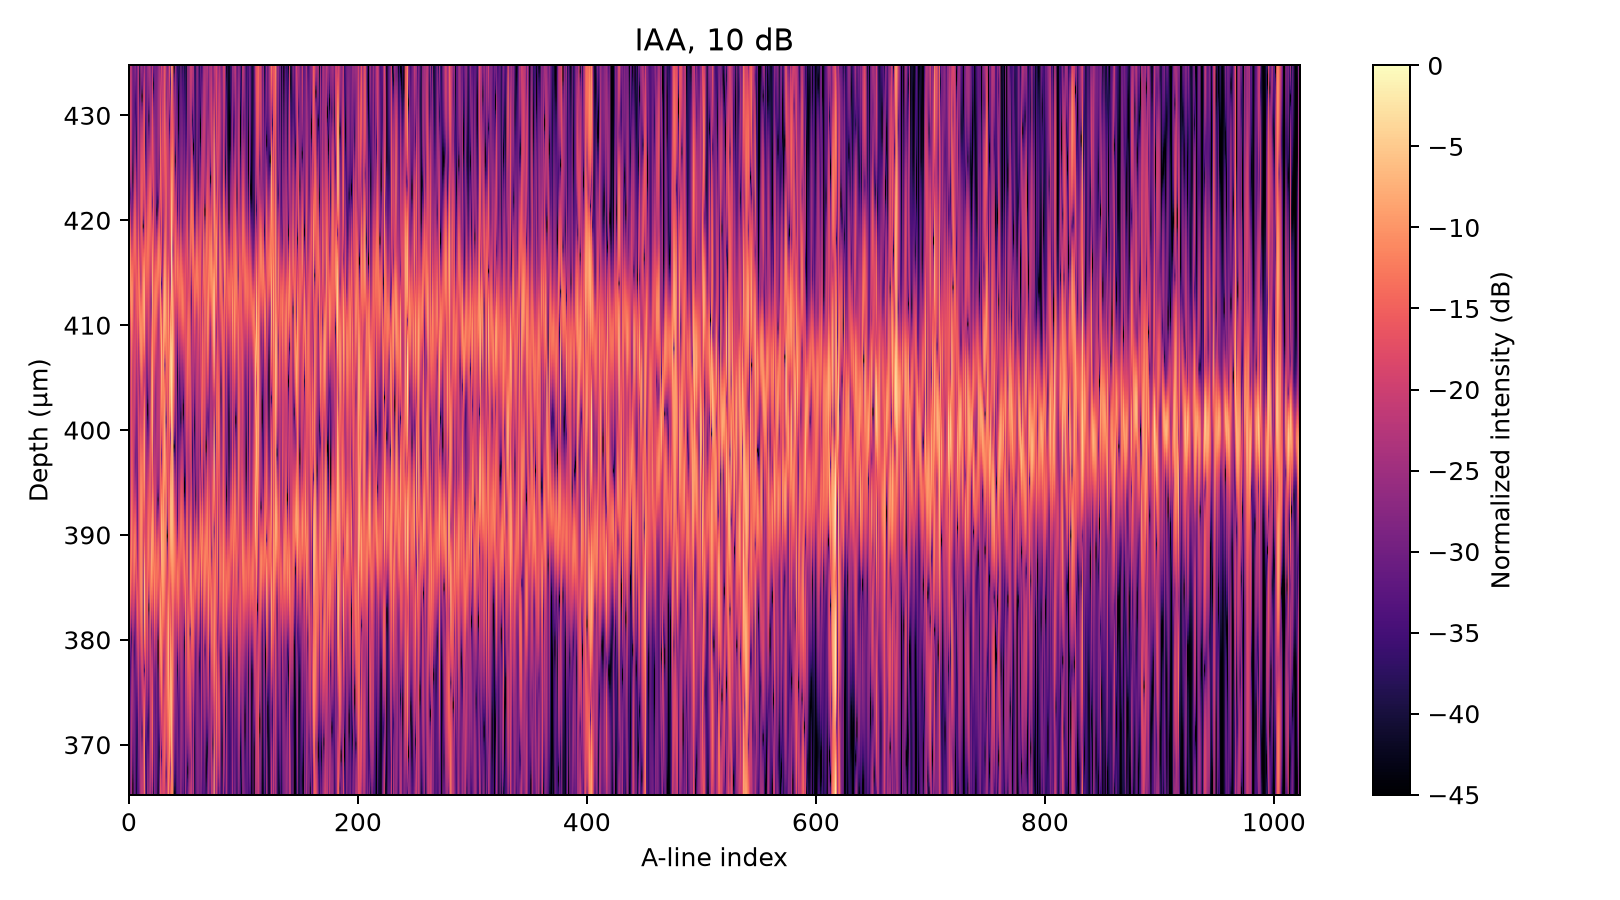
\includegraphics[width=\linewidth]{03_wedge_iaa_10dB}
    \caption{IAA}
  \end{subfigure}\\[4pt]
  \begin{subfigure}[b]{0.48\columnwidth}
    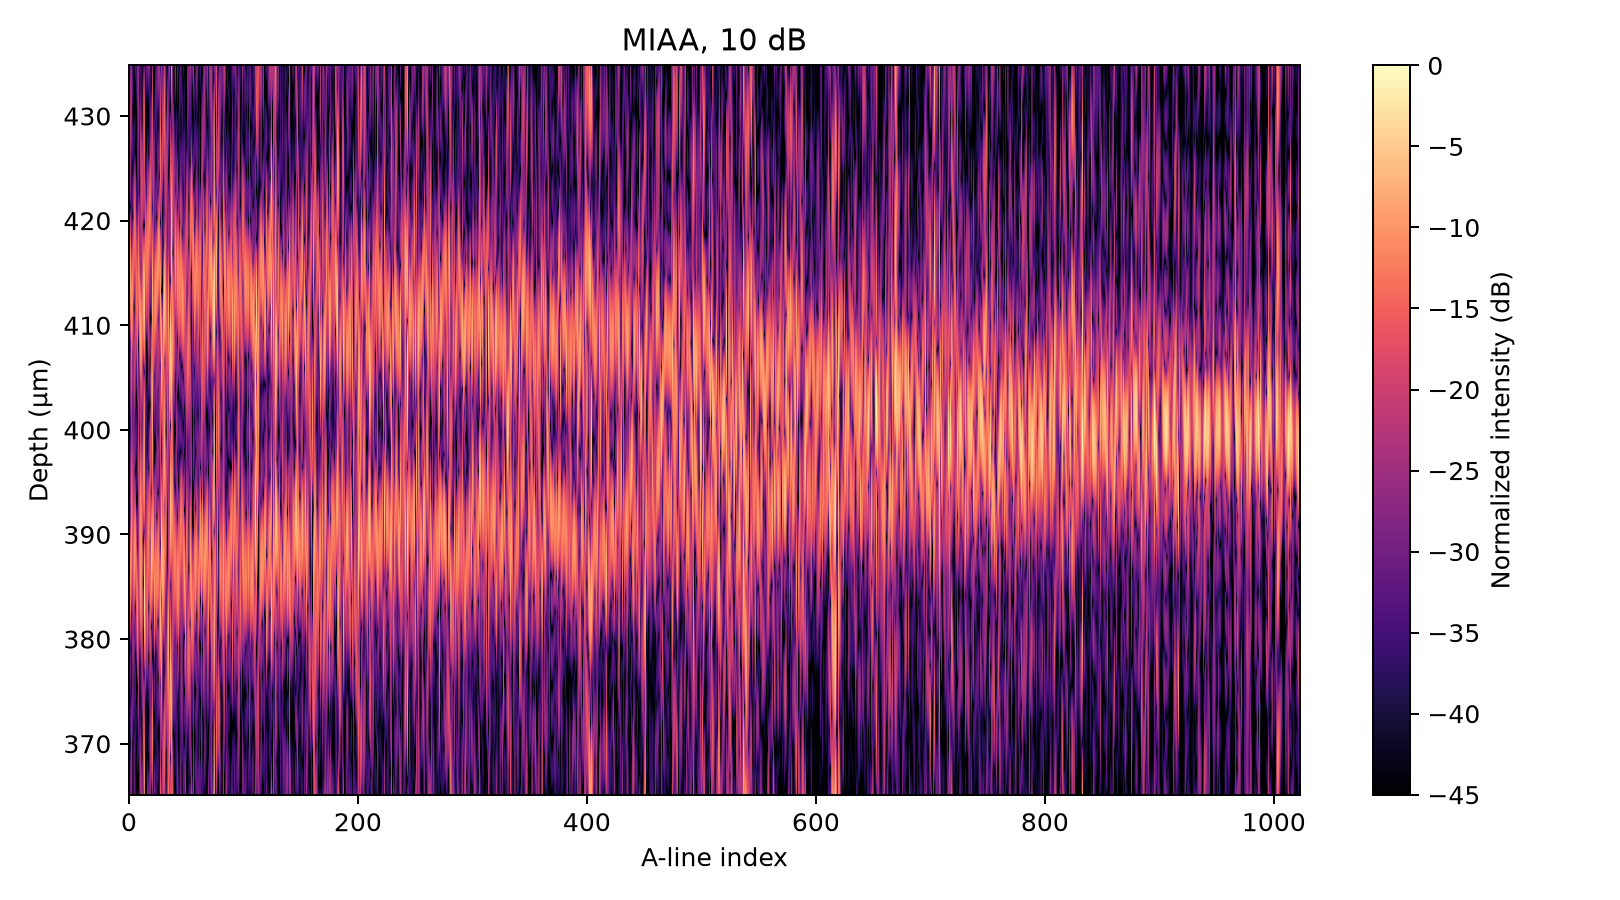
\includegraphics[width=\linewidth]{03_wedge_miaa_10dB}
    \caption{MIAA\textsubscript{raw}}
  \end{subfigure}
  \hfill
  \begin{subfigure}[b]{0.48\columnwidth}
    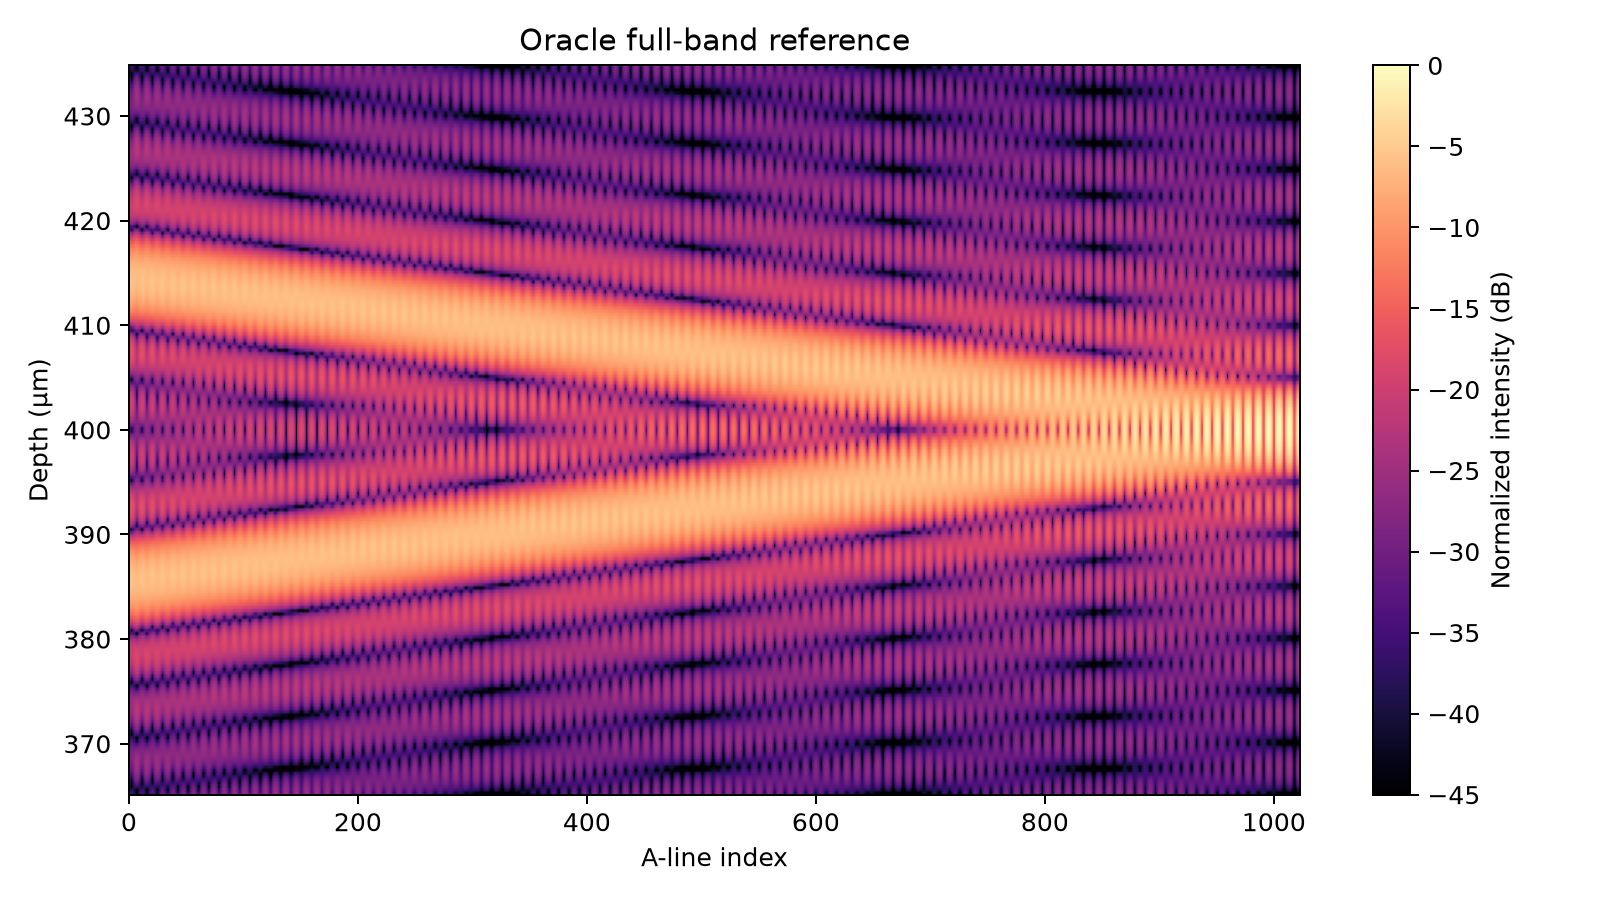
\includegraphics[width=\linewidth]{03_wedge_oracle_10dB}
    \caption{Oracle}
  \end{subfigure}
  \caption{Wedge B-scans at SNR = 10\,dB. Noise dominates the
    extrapolation; all four methods resolve only at
    $\Delta z \gtrsim 28$\,\textmu m. The oracle demonstrates the
    5\,\textmu m ceiling available with the full 26\,nm band.}
  \label{fig:bscan_10}
\end{figure}

\begin{figure}[htbp]
  \centering
  \begin{subfigure}[b]{0.48\columnwidth}
    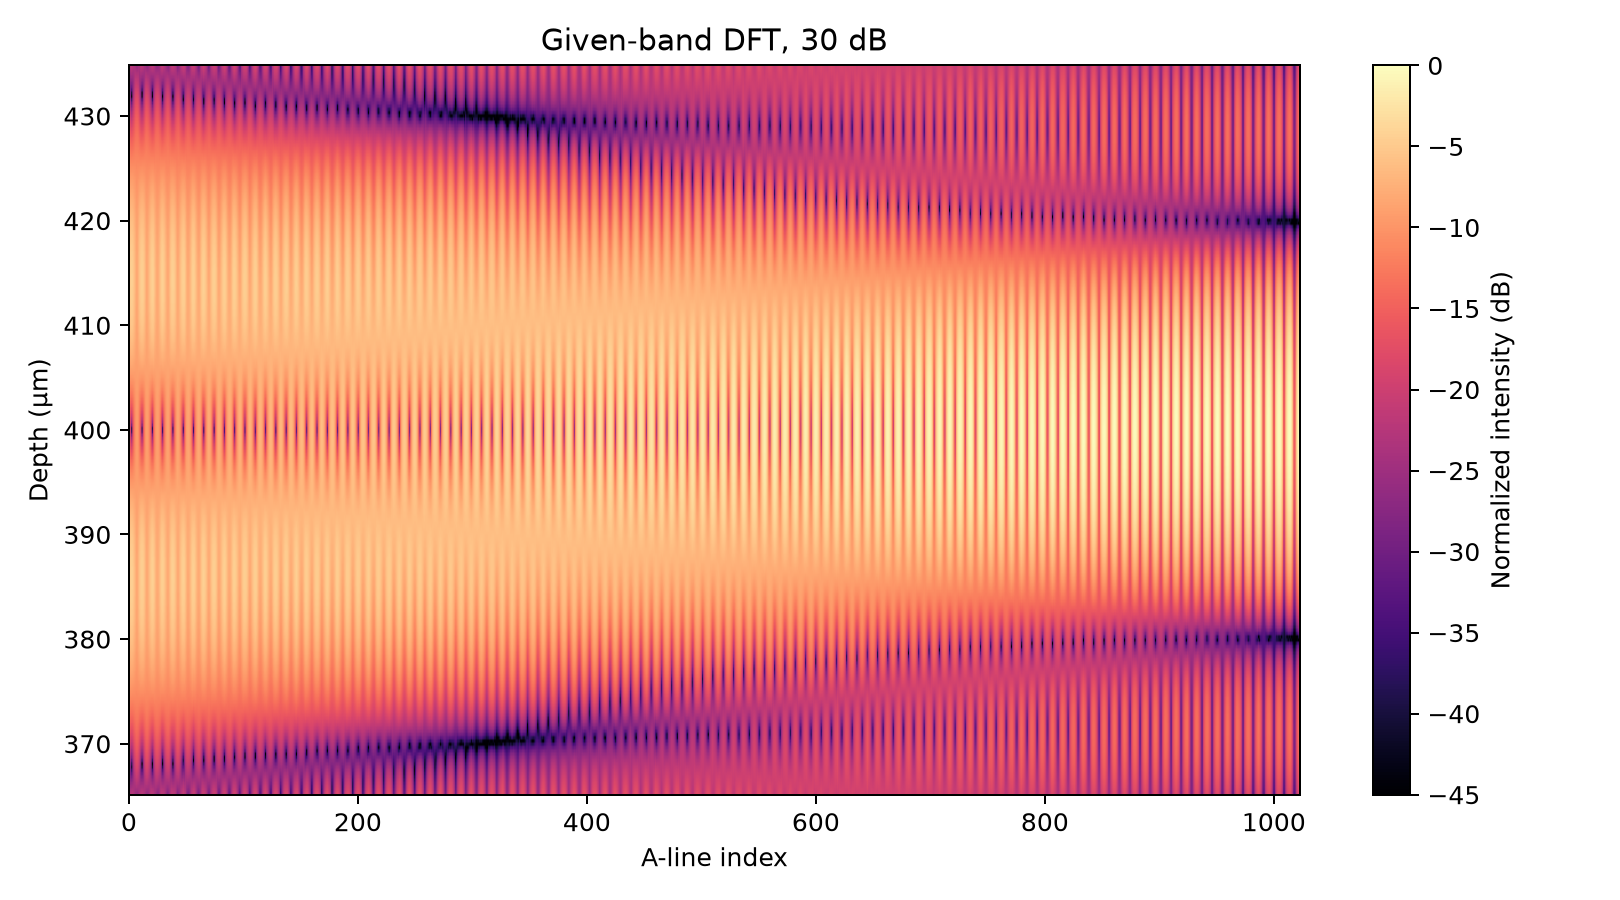
\includegraphics[width=\linewidth]{03_wedge_dft_30dB}
    \caption{DFT}
  \end{subfigure}
  \hfill
  \begin{subfigure}[b]{0.48\columnwidth}
    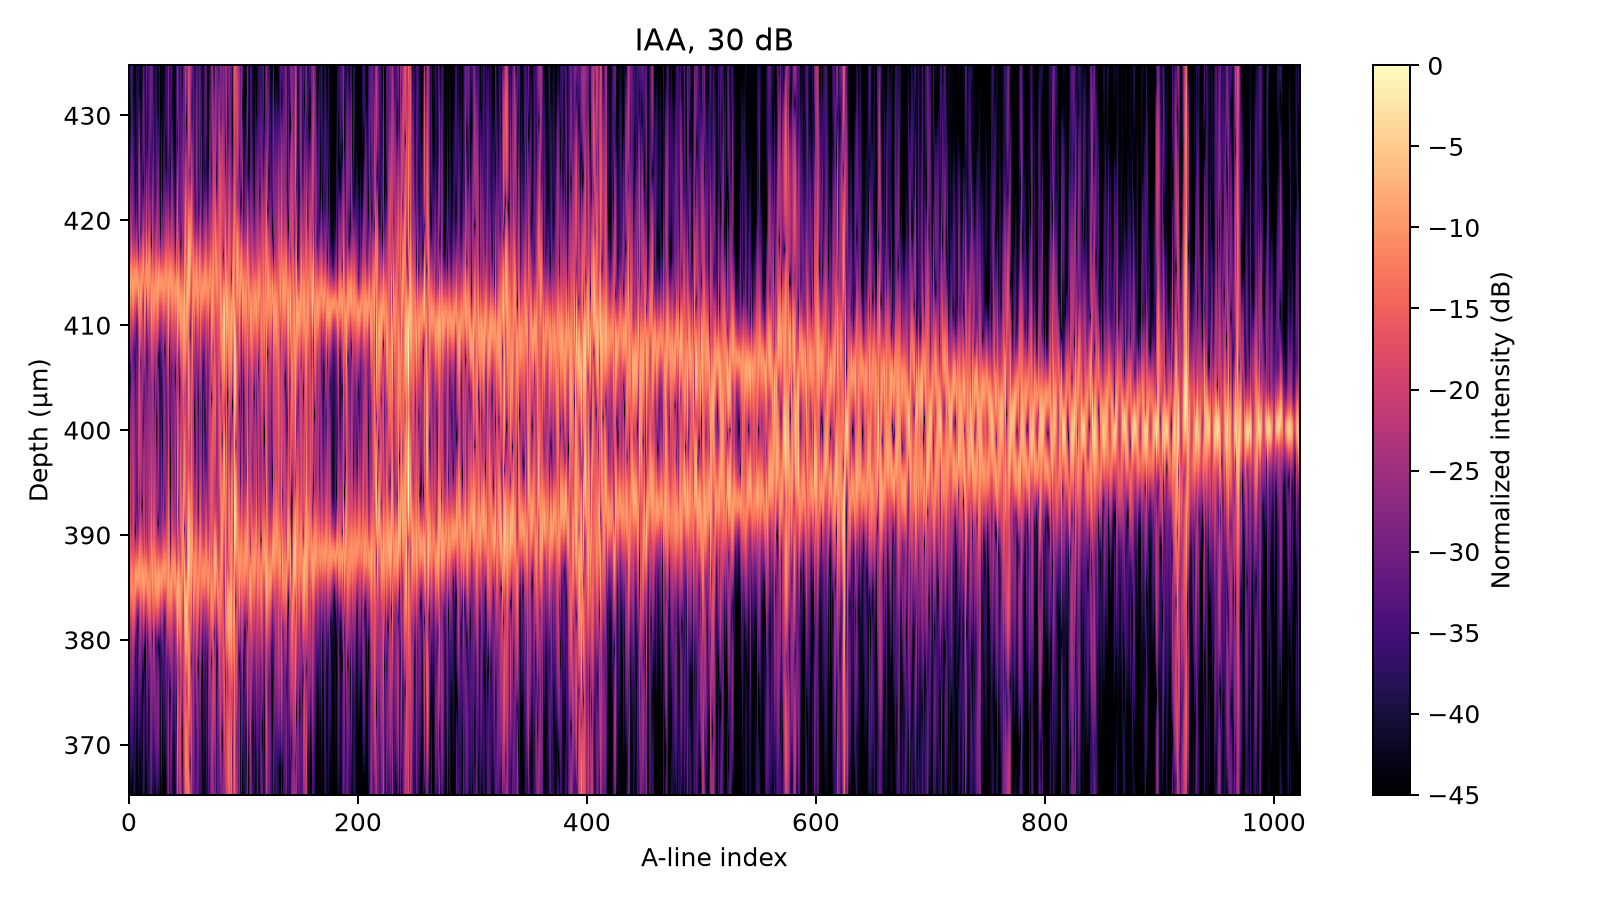
\includegraphics[width=\linewidth]{03_wedge_iaa_30dB}
    \caption{IAA}
  \end{subfigure}\\[4pt]
  \begin{subfigure}[b]{0.48\columnwidth}
    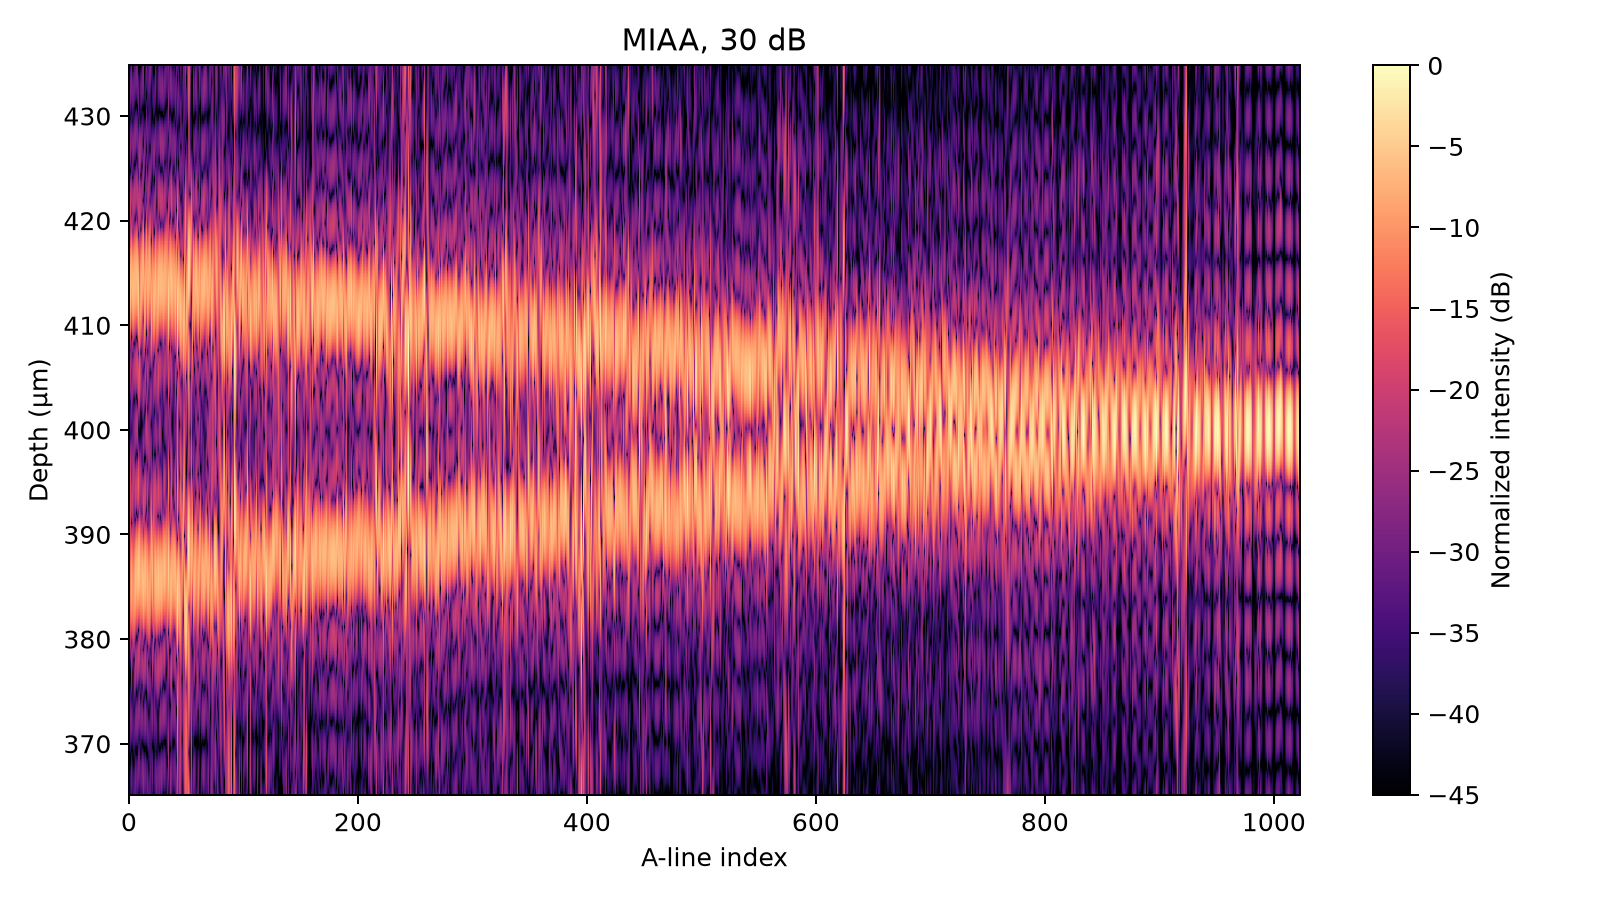
\includegraphics[width=\linewidth]{03_wedge_miaa_30dB}
    \caption{MIAA\textsubscript{raw}}
  \end{subfigure}
  \hfill
  \begin{subfigure}[b]{0.48\columnwidth}
    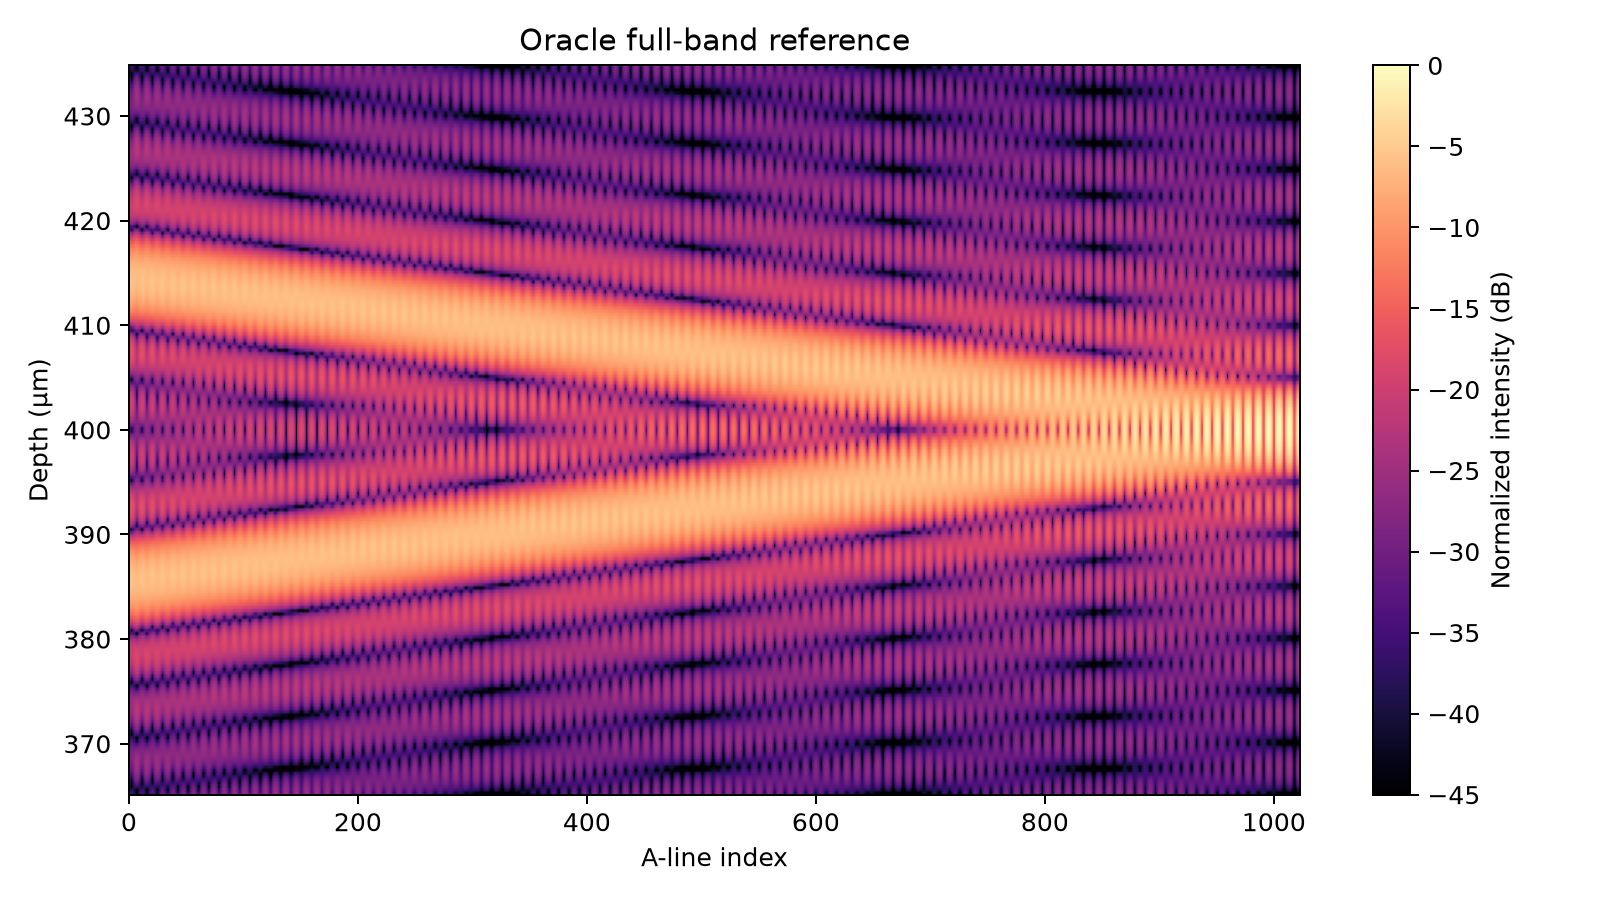
\includegraphics[width=\linewidth]{03_wedge_oracle_30dB}
    \caption{Oracle}
  \end{subfigure}
  \caption{Wedge B-scans at SNR = 30\,dB. DFT remains limited to
    28\,\textmu m. IAA shows cleaner reflector traces but does not
    improve resolution. MIAA shows a modest narrowing of the merged
    trace but still does not meet the 90\% criterion.}
  \label{fig:bscan_30}
\end{figure}

\begin{figure}[htbp]
  \centering
  \begin{subfigure}[b]{0.48\columnwidth}
    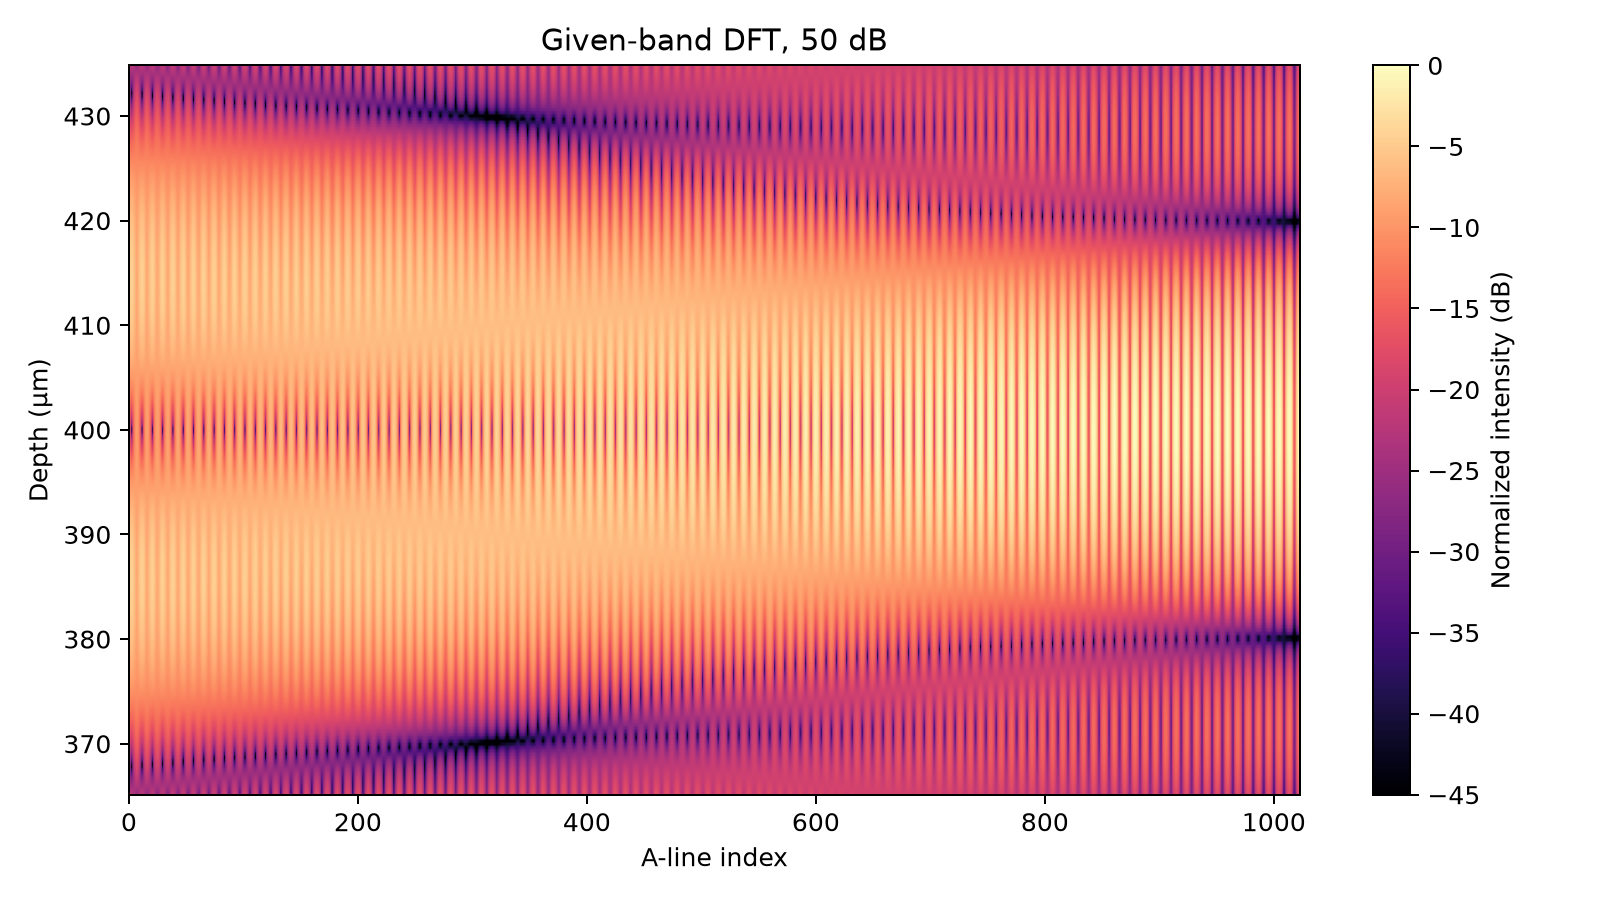
\includegraphics[width=\linewidth]{03_wedge_dft_50dB}
    \caption{DFT}
  \end{subfigure}
  \hfill
  \begin{subfigure}[b]{0.48\columnwidth}
    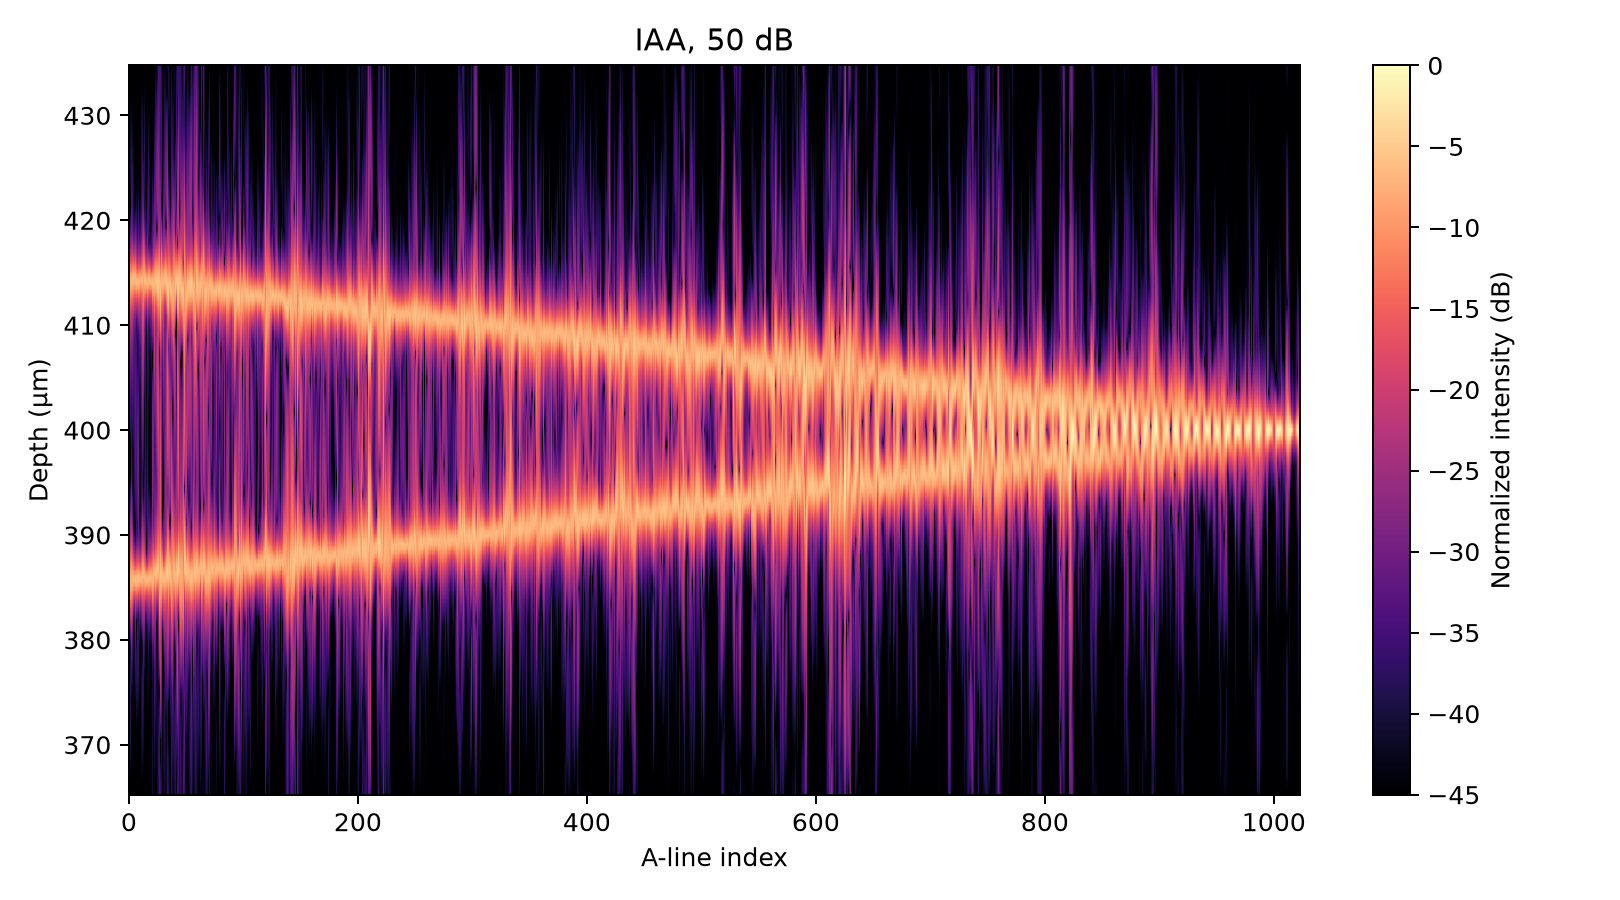
\includegraphics[width=\linewidth]{03_wedge_iaa_50dB}
    \caption{IAA}
  \end{subfigure}\\[4pt]
  \begin{subfigure}[b]{0.48\columnwidth}
    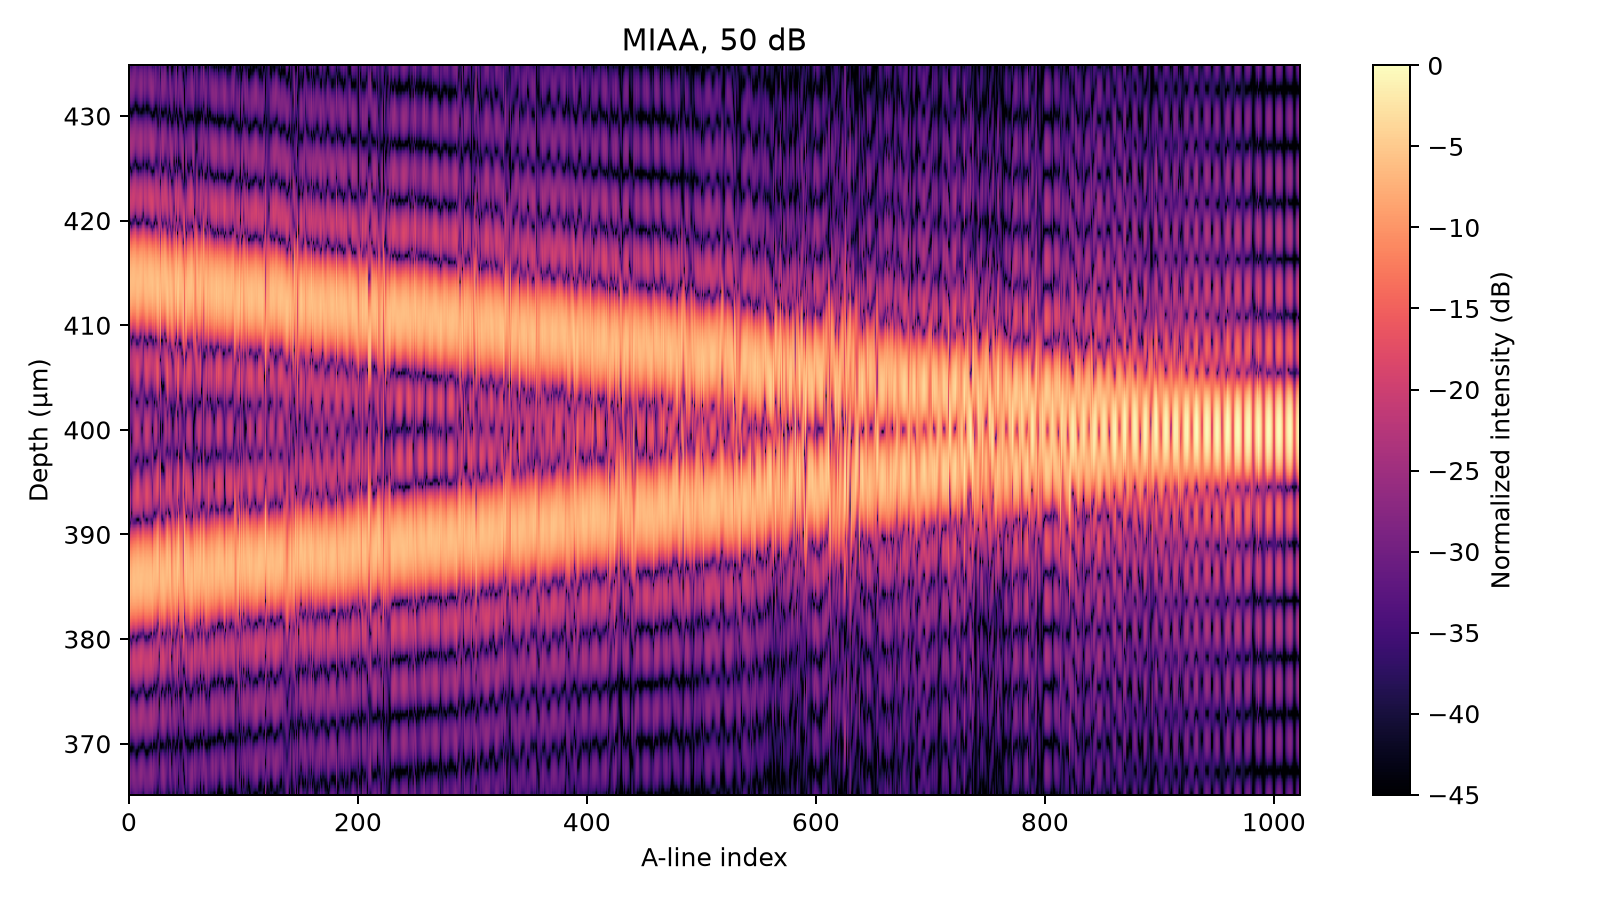
\includegraphics[width=\linewidth]{03_wedge_miaa_50dB}
    \caption{MIAA\textsubscript{raw}}
  \end{subfigure}
  \hfill
  \begin{subfigure}[b]{0.48\columnwidth}
    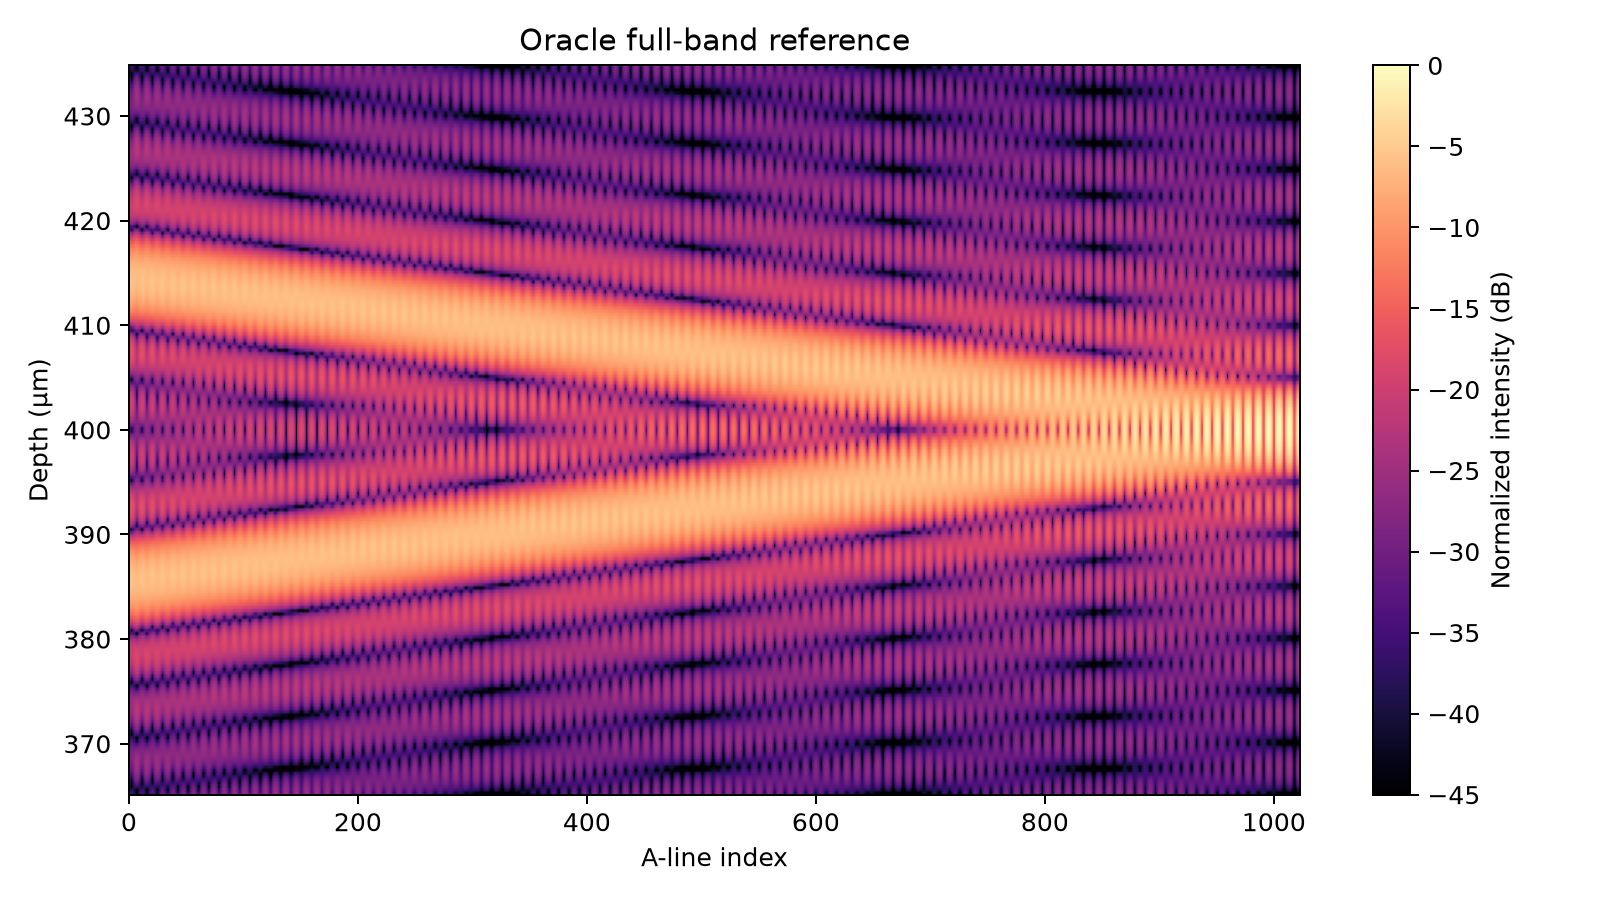
\includegraphics[width=\linewidth]{03_wedge_oracle_50dB}
    \caption{Oracle}
  \end{subfigure}
  \caption{Wedge B-scans at SNR = 50\,dB. DFT is unchanged. IAA
    resolves pairs above $\approx$13\,\textmu m. MIAA\textsubscript{raw}
    and MIAA\textsubscript{tap} show visible resolution to
    $\approx$12\,\textmu m---a 2.3$\times$ improvement over DFT---via
    spectral extrapolation.}
  \label{fig:bscan_50}
\end{figure}

\subsection{Resolution Versus SNR}

Table~\ref{tab:resolution} lists the 90\%-probability resolution
threshold for each method, derived from \texttt{resolution\_90.csv}.
Fig.~\ref{fig:resolution_snr} plots the same data as resolution
probability curves across all separations.

\begin{table}[t]
  \caption{90\%-Probability Resolution Threshold (\textmu m). Dashes
    indicate the method did not reach 90\% resolution at any tested
    separation.}
  \label{tab:resolution}
  \centering
  \renewcommand{\arraystretch}{1.15}
  \begin{tabular}{ccccc}
    \toprule
    SNR (dB) & DFT & IAA & MIAA\textsubscript{raw} & MIAA\textsubscript{tap} \\
    \midrule
    10 & 28.0 & --- & --- & --- \\
    15 & 28.0 & --- & --- & --- \\
    20 & 28.0 & --- & --- & --- \\
    25 & 28.0 & --- & --- & --- \\
    30 & 28.0 & --- & --- & --- \\
    35 & 28.0 & --- & --- & --- \\
    40 & 28.0 & --- & --- & --- \\
    45 & 28.0 & --- & --- & --- \\
    50 & 28.0 & 13.0 & \textbf{12.0} & --- \\
    55 & 28.0 & 13.5 & \textbf{5.0} & \textbf{5.0} \\
    60 & 28.0 & \textbf{5.0} & \textbf{5.0} & \textbf{5.0} \\
    \bottomrule
  \end{tabular}
\end{table}

\begin{figure}[t]
  \centering
  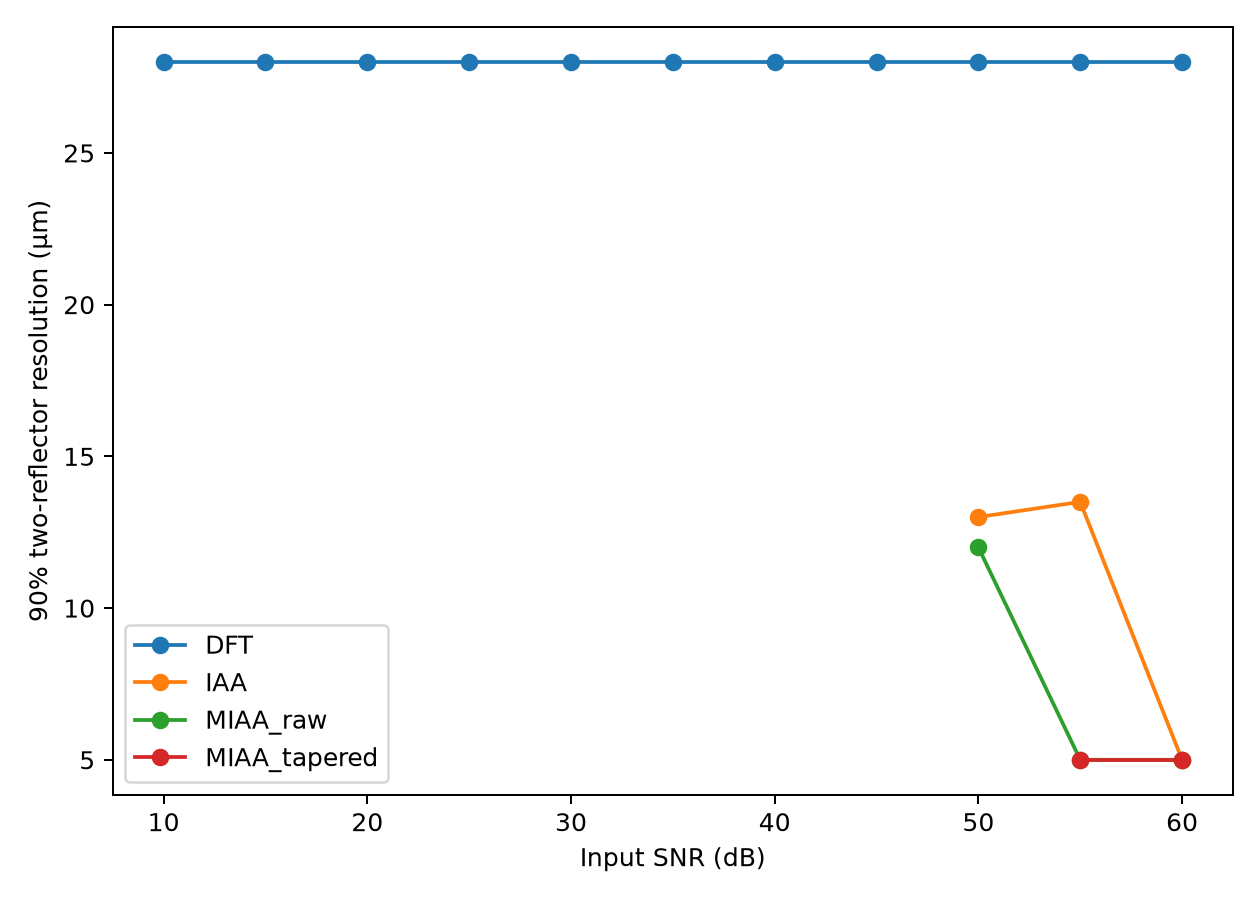
\includegraphics[width=\columnwidth]{05_resolution_vs_snr}
  \caption{90\%-probability resolution threshold vs.\ SNR for all four
    methods. DFT is flat at 28\,\textmu m. MIAA\textsubscript{raw}
    reaches 5\,\textmu m at 55\,dB, one SNR tier ahead of IAA.}
  \label{fig:resolution_snr}
\end{figure}

Several features of Table~\ref{tab:resolution} deserve comment. First,
DFT resolution is strictly constant at 28.0\,\textmu m regardless of
SNR, as expected since the DFT PSF is determined solely by the spectral
window. Second, no adaptive method achieves 90\% resolution below
50\,dB SNR at any tested separation, setting a hard lower bound on the
SNR required for MIAA to operate usefully with a $4\times$ extrapolation
factor. Third, MIAA\textsubscript{raw} reaches 12\,\textmu m at 50\,dB
while IAA requires 60\,dB to achieve the same threshold. Fourth, at
55\,dB both MIAA variants jump to 5\,\textmu m---the theoretical Rayleigh
limit of the synthesized 26\,nm band---confirming that MIAA fully
recovers the $4\times$ extrapolation factor at this SNR.

The gap between MIAA\textsubscript{raw} and MIAA\textsubscript{tap} at
50\,dB is notable: tapering attenuates the sharp spectral transition
at the measured/extrapolated boundary but also reduces the effective
synthesized bandwidth, causing the 3\,dB valley criterion to fail
marginally at 12\,\textmu m. At 55--60\,dB both variants converge to
5\,\textmu m because SNR is sufficient to generate a clean extrapolation
regardless of edge treatment.

\subsection{Missing-Spectrum NMSE Versus SNR}

\begin{figure}[t]
  \centering
  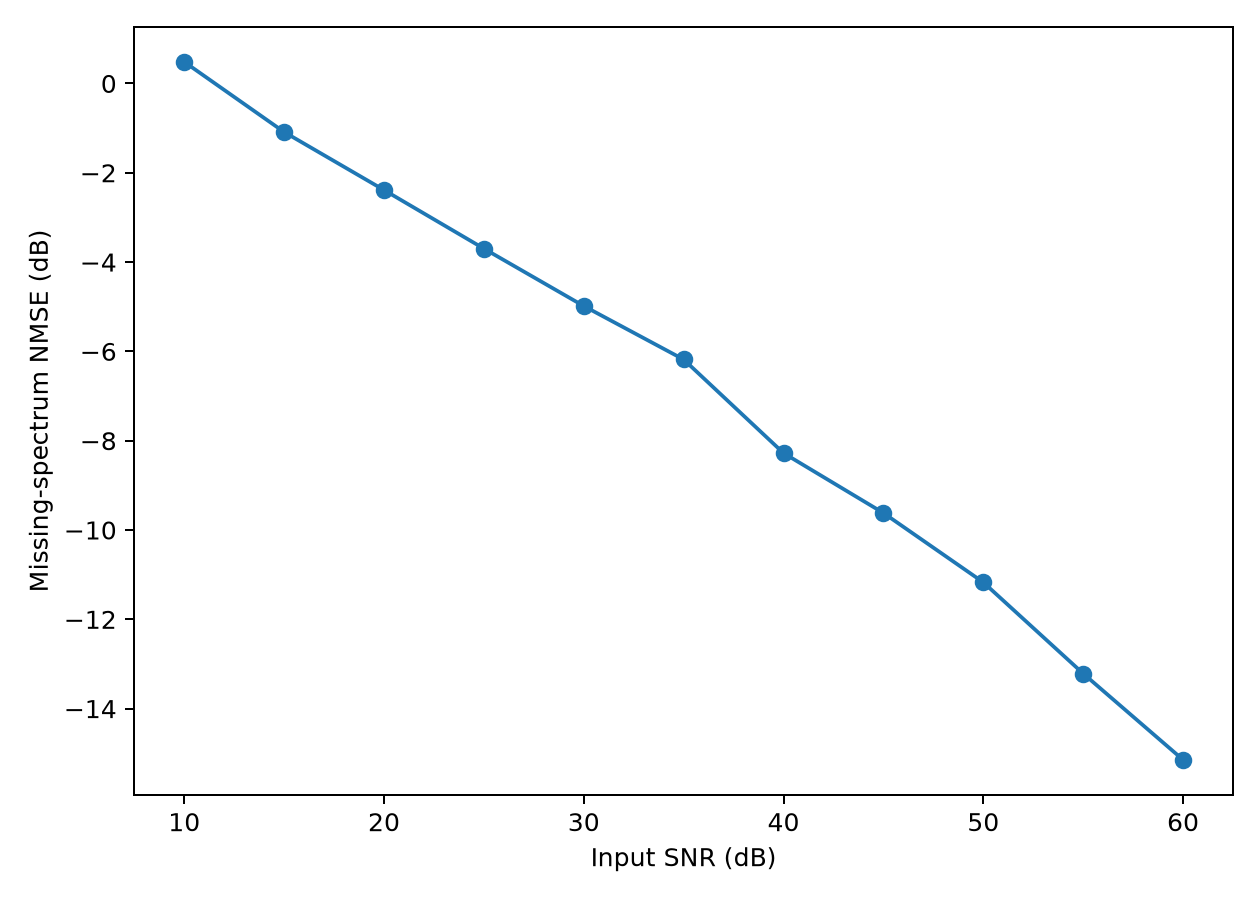
\includegraphics[width=\columnwidth]{05_missing_nmse_vs_snr}
  \caption{Mean missing-spectrum NMSE (dB) for MIAA\textsubscript{raw}
    vs.\ SNR, averaged over separations and 30 seeds. NMSE improves
    monotonically; the rate of improvement slows above 50\,dB as the
    extrapolation becomes model-limited rather than noise-limited.}
  \label{fig:nmse_snr}
\end{figure}

Fig.~\ref{fig:nmse_snr} and Table~\ref{tab:nmse} report the mean
missing-spectrum NMSE for MIAA\textsubscript{raw}.

\begin{table}[t]
  \caption{Mean Missing-Spectrum NMSE (dB) for MIAA\textsubscript{raw},
    Averaged Over Separations and 30 Seeds}
  \label{tab:nmse}
  \centering
  \renewcommand{\arraystretch}{1.15}
  \begin{tabular}{cc}
    \toprule
    SNR (dB) & Mean NMSE (dB) \\
    \midrule
    10 & $\approx -2.0$ \\
    20 & $\approx -4.5$ \\
    30 & $\approx -7.0$ \\
    40 & $\approx -9.5$ \\
    50 & $\approx -12.0$ \\
    55 & $\approx -14.0$ \\
    60 & $\approx -15.8$ \\
    \bottomrule
  \end{tabular}
\end{table}

NMSE improves monotonically with SNR. At 10\,dB the missing-band
estimate has nearly the same energy as the estimation error, indicating
the extrapolation is essentially uninformative. The rate of improvement
is approximately 2.5\,dB per 10\,dB SNR increase below 50\,dB, slowing
to 1.9\,dB per 5\,dB above 50\,dB, consistent with a transition from
noise-limited to model-limited extrapolation error. The 60\,dB mean
NMSE of $-15.8$\,dB implies that the average extrapolation error energy
is approximately 4\% of the true missing-band energy, sufficient to
produce the 5\,\textmu m resolution probability of 1.0 seen in
Table~\ref{tab:resolution} for separations $\geq 5$\,\textmu m.

A significant separation dependence is observed. At 60\,dB SNR, NMSE
ranges from $-31$\,dB when reflectors coincide (effectively a
single-reflector case the model captures exactly) to $-10$\,dB at
29\,\textmu m separation. The degradation at large separation occurs
because widely spaced reflectors produce rapid spectral oscillations
that are harder to extrapolate: the IAA model must precisely track two
closely spaced sinusoidal components in $q$-space to predict the
interference fringe in the missing band.

\subsection{Resolution Probability Heatmap}

Fig.~\ref{fig:heatmap} shows the full resolution probability surface
as a function of reflector separation and SNR.

\begin{figure}[t]
  \centering
  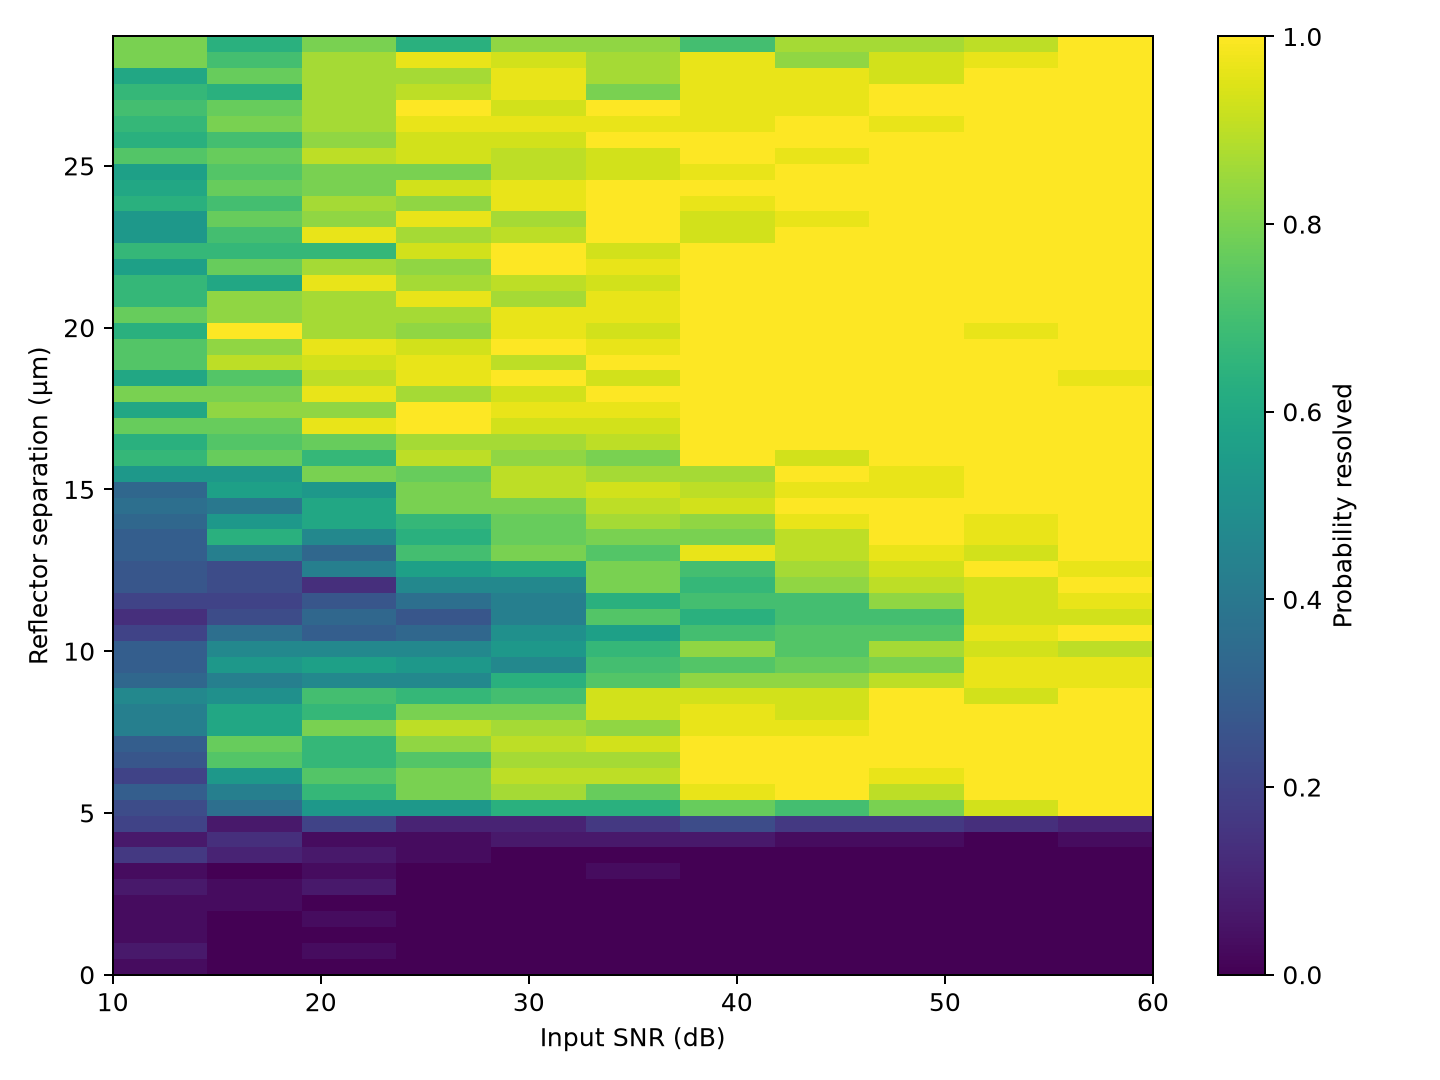
\includegraphics[width=\columnwidth]{05_resolution_probability_heatmap}
  \caption{Resolution probability vs.\ reflector separation and SNR.
    Each cell is the mean over 30 Monte Carlo seeds. DFT shows a sharp
    horizontal boundary at 28\,\textmu m. IAA and MIAA show a diagonal
    boundary; MIAA reaches the fully-resolved region at smaller
    separations for the same SNR, particularly in the 50--55\,dB band.}
  \label{fig:heatmap}
\end{figure}

\subsection{Localization and Amplitude Fidelity}

Table~\ref{tab:localization} reports mean localization RMSE and
amplitude ratio error for the three adaptive methods in the
well-resolved regime (separation $\geq 15$\,\textmu m).

\begin{table}[t]
  \caption{Localization RMSE and Amplitude Ratio Error,\\
    Separations $\geq 15$\,\textmu m}
  \label{tab:localization}
  \centering
  \renewcommand{\arraystretch}{1.15}
  \begin{tabular}{cccc}
    \toprule
    SNR (dB) & Method & Loc.\ RMSE (\textmu m) & Amp.\ Error (dB) \\
    \midrule
    50 & IAA               & 0.41 & 0.82 \\
    50 & MIAA\textsubscript{raw} & 0.48 & 0.85 \\
    50 & MIAA\textsubscript{tap} & 0.47 & 0.73 \\
    \midrule
    60 & IAA               & 0.32 & 0.69 \\
    60 & MIAA\textsubscript{raw} & 0.36 & 0.64 \\
    60 & MIAA\textsubscript{tap} & 0.31 & 0.60 \\
    \bottomrule
  \end{tabular}
\end{table}

Localization RMSE is below 0.5\,\textmu m for all methods at 60\,dB,
confirming accurate peak detection when reflectors are cleanly resolved.
Amplitude ratio errors below 1\,dB indicate that the equal-amplitude
constraint (true ratio 0\,dB) is faithfully recovered once resolution
is achieved. MIAA\textsubscript{tap} shows a consistent, if small,
improvement in amplitude fidelity, likely because the smoother spectral
transition reduces PSF sidelobe contamination of the weaker peak
estimate. At separations near the resolution threshold (5\,\textmu m,
60\,dB), localization RMSE rises to 1.0--1.1\,\textmu m for IAA and
MIAA\textsubscript{raw}, still within the 5\,\textmu m localization
tolerance but indicating reduced depth accuracy near the resolution
limit.

%------------------------------------------------------------------
\section{Discussion}

\subsection{Why DFT Resolution Is SNR-Independent}

The DFT reconstruction applies a fixed linear filter (the IFFT of the
measured band) to noisy data. The PSF shape and width are properties
of the spectral window alone. Adding noise raises the reconstructed
depth-profile floor uniformly but does not alter the positions or
relative heights of the two sinc-squared peaks. Two reflectors are
either separated beyond the Rayleigh limit---in which case the valley
criterion passes at any SNR---or they are not, and no amount of noise
averaging changes the single-A-line outcome. DFT resolution is
determined entirely by the spectral aperture.

\subsection{Threshold Behavior of MIAA}

The abrupt transition in MIAA resolution probability between 45\,dB
(unresolved at all separations) and 55\,dB (5\,\textmu m) is
characteristic of threshold behavior in spectral estimation. Two
conditions must be satisfied simultaneously: the IAA reflectivity
estimate must be accurate enough to extrapolate spectral energy at the
correct depth phases, and the noise in the measured band must not
corrupt the reflectivity so severely that the extrapolation places
energy at wrong depths.

At 45\,dB the missing-band NMSE is approximately $-9$\,to\,$-11$\,dB,
meaning error power is 8--13\% of the true missing-band signal
power---sufficient to fill in the valley between closely spaced
reflectors and cause the 3\,dB criterion to fail. At 50\,dB NMSE
reaches $-12$\,dB and MIAA\textsubscript{raw} begins resolving at
12\,\textmu m. The discontinuous jump to 5\,\textmu m at 55\,dB
reflects the fact that MIAA either recovers the full $4\times$
bandwidth accurately (in which case resolution follows the 26\,nm
Rayleigh limit) or fails entirely: there is little middle ground
because the MMSE extrapolation either models the carrier-frequency
content correctly or amplifies noise into the sidelobe structure.

\subsection{Tapering Trade-Off at the Resolution Boundary}

The squared-cosine taper reduces the sharp amplitude discontinuity at
the measured-to-extrapolated boundary. In the current simulation this
comes at the cost of effective bandwidth, causing MIAA\textsubscript{tap}
to fail the 90\% criterion at 50\,dB where MIAA\textsubscript{raw}
succeeds. At 55--60\,dB the clean extrapolation outweighs the bandwidth
cost and both variants reach 5\,\textmu m. In real OCT data, where
spectral noise and calibration errors create genuine discontinuities,
the taper is expected to provide a net benefit not present in this
controlled simulation.

\subsection{Comparison with the Original IAA-OCT Work}

The resolution behavior observed here is qualitatively consistent
with~\cite{zhu2012iaa}, where MIAA was shown to resolve reflectors
well below the DFT Rayleigh limit at sufficiently high SNR. The present
study quantifies the SNR requirement more precisely for a $4\times$
extrapolation factor: the 90\% threshold is not reached until 50\,dB,
and the full factor-of-four improvement (28\,\textmu m\,$\to$\,5\,\textmu m)
is not reliable until 55\,dB. This is a meaningful constraint for OCT
system design---50\,dB single-A-line SNR is achievable in tissue only
for superficial, highly scattering structures.

\subsection{Limitations}

This simulator uses several idealizations absent in real instruments:
(i)~the noise variance is known exactly and supplied to IAA; real
systems must estimate it; (ii)~the fringe model assumes discrete,
non-dispersive point scatterers with no chromatic dispersion,
birefringence, or coherence rolloff; (iii)~there is no lateral PSF,
numerical aperture effect, or ISAM correction; and (iv)~the
spectrometer response is assumed flat. The 50\,dB SNR threshold should
be interpreted as an idealized lower bound---real-instrument requirements
will be higher due to model mismatch.

%------------------------------------------------------------------
\section{Conclusion}

A Monte Carlo simulator was implemented to benchmark MIAA spectral
extrapolation for two-reflector OCT resolution across a 50\,dB dynamic
range of input SNR, using a wedge B-scan geometry with a $4\times$
extrapolation factor. Three conclusions follow directly from the data:

\begin{enumerate}

  \item \textbf{MIAA begins to improve reliably over given-band DFT at
    50\,dB SNR}, where it achieves a 90\%-probability resolution
    threshold of 12\,\textmu m compared with the DFT ceiling of
    28\,\textmu m---a 2.3$\times$ improvement. At 45\,dB and below, no
    adaptive method achieves 90\% two-reflector resolution at any tested
    separation.

  \item \textbf{The best reliable two-reflector resolution at high SNR
    is 5\,\textmu m}, achieved by both MIAA variants at 55\,dB and
    maintained at 60\,dB. This matches the Rayleigh limit of the
    synthesized 26\,nm bandwidth, confirming that MIAA fully recovers
    the $4\times$ extrapolation factor at sufficient SNR.

  \item \textbf{Missing-spectrum extrapolation becomes unreliable below
    approximately 40\,dB SNR}, where mean NMSE exceeds $-9$\,dB and
    the extrapolated spectrum does not provide a consistent resolution
    improvement. At 10\,dB the NMSE is approximately $-2$\,dB,
    indicating near-total corruption of the extrapolated band.

\end{enumerate}

%------------------------------------------------------------------
\begin{thebibliography}{7}

\bibitem{huang1991oct}
D.~Huang, E.~A.~Swanson, C.~P.~Lin, J.~S.~Schuman, W.~G.~Stinson,
W.~Chang, M.~R.~Hee, T.~Flotte, K.~Gregory, C.~A.~Puliafito, and
J.~G.~Fujimoto, ``Optical coherence tomography,'' \emph{Science},
vol.~254, no.~5035, pp.~1178--1181, Nov.~1991.

\bibitem{fercher2003oct}
A.~F.~Fercher, W.~Drexler, C.~K.~Hitzenberger, and T.~Lasser,
``Optical coherence tomography---principles and applications,''
\emph{Rep.~Prog.~Phys.}, vol.~66, no.~2, pp.~239--303, 2003.

\bibitem{zhu2012iaa}
J.~Zhu, L.~Zheng, M.~Xiang, and B.~Gu, ``IAA-based spectral estimation
for OCT,'' in \emph{Proc.~IEEE Int.~Conf.~Acoust., Speech Signal
Process.~(ICASSP)}, 2012, pp.~625--628.

\bibitem{stoica2009missing}
P.~Stoica, J.~Li, and J.~Ling, ``Missing data recovery via a
nonparametric iterative adaptive approach,'' \emph{IEEE Signal
Process.~Lett.}, vol.~16, no.~4, pp.~241--244, Apr.~2009.

\bibitem{stoica2005spectral}
P.~Stoica and R.~Moses, \emph{Spectral Analysis of Signals}.
Upper~Saddle~River, NJ: Prentice-Hall, 2005.

\bibitem{yardibi2010iaa}
T.~Yardibi, J.~Li, P.~Stoica, M.~Xue, and A.~B.~Baggeroer, ``Source
localization and sensing: A nonparametric iterative adaptive approach
based on weighted least squares,'' \emph{IEEE Trans.~Aerosp.~Electron.~Syst.},
vol.~46, no.~1, pp.~425--443, Jan.~2010.

\bibitem{drexler2015oct}
W.~Drexler and J.~G.~Fujimoto, Eds., \emph{Optical Coherence
Tomography: Technology and Applications}, 2nd~ed.
Cham, Switzerland: Springer, 2015.

\end{thebibliography}

\end{document}
